% 自动控制理论 课程笔记 —— 优化版主文件
% 编译环境：XeLaTeX（必须！）
% 无多余警告，支持书签中文，增加常用环境

\documentclass[oneside,UTF8]{ctexbook}

% ========== 核心宏包（有序加载） ==========
\usepackage{amsmath, amssymb, amsfonts}
\usepackage{amsthm}          % 定理环境
\usepackage{graphicx}
\usepackage{geometry}
\usepackage{url}
\usepackage{booktabs}
\usepackage{enumitem}
\usepackage{xcolor}
\usepackage{tcolorbox}
\tcbuselibrary{skins}
\usepackage{tikz}
\usepackage{etoolbox}
\usepackage{titlesec}
\usepackage{fancyhdr}        % 页眉页脚
\usepackage{listings}        % 代码环境（可选）
\usepackage{silence}

% ========== 页面设置 ==========
\geometry{
    a4paper, left=2.5cm, right=2.5cm,
    top=2.5cm, bottom=2.5cm, headheight=15pt
}

% ========== 屏蔽可控警告 ==========
\hbadness=10000
\vfuzz=10pt
\hfuzz=10pt
\WarningFilter{xeCJK}{Redefining CJKfamily}
\WarningFilter{LaTeX Font}{Some font shapes were not available}
\WarningFilter{hyperref}{Token not allowed}
\WarningFilter{hyperref}{Unsupported document}
\WarningFilter{enumitem}{Negative labelwidth}  % 可选

% ========== 目录深度 ==========
\setcounter{tocdepth}{2}
\setcounter{secnumdepth}{3}

% ========== 章节标题样式（修正） ==========
\titleformat{\chapter}
    {\centering\bfseries\Large\zihao{-2}}   % 若无效可改用 \fontsize{18pt}{22pt}\selectfont
    {第\thechapter 章}
    {0.5em}
    {}

\titleformat{\section}
    {\bfseries\large\zihao{-3}}
    {\thesection}
    {0.5em}
    {}

\titleformat{\subsection}
    {\bfseries\normalsize\zihao{4}}
    {\thesubsection}
    {0.5em}
    {}

% ========== 列表间距 ==========
\setlist{leftmargin=2em, itemsep=0.2em, parsep=0pt}

% ========== 页眉页脚（已修复 oneside 警告）==========
\pagestyle{fancy}
\fancyhf{}
\fancyhead[L]{\leftmark}
\fancyhead[R]{\rightmark}
\fancyfoot[C]{\thepage}
\renewcommand{\headrulewidth}{0.4pt}

% ========== 数学定理环境 ==========
\theoremstyle{definition}
\newtheorem{definition}{定义}[section]
\newtheorem{theorem}{定理}[section]
\newtheorem{example}{例}[section]

% ========== 超链接（最佳配置） ==========
\usepackage[
    colorlinks = true,
    linkcolor  = blue,
    citecolor  = blue,
    urlcolor   = blue,
    linktoc    = all,
    pdfencoding=auto,
    psdextra   = true          % 增强 PDF 字符串处理
]{hyperref}

\hypersetup{
    pdftitle={自动控制理论课程笔记},
    pdfauthor={2024级电气工程及其自动化},
    pdfsubject={自动控制理论},
    pdfkeywords={自控, 时域, 频域, 根轨迹}
}

% 仅屏蔽书签中的数学模式常见警告
\pdfstringdefDisableCommands{%
    \let\(\(%
    \let\)\)%
    \def\underscore{\_}%
}

% ========== 文档信息 ==========
\title{自动控制理论（EE3003）课程笔记}
\author{2024级电气工程及其自动化专业}
\date{2026 春季学期}

\xeCJKDeclareCharClass{CJK}{"2460->"24FF, "2160->"217F}

\begin{document}

% 封面定义（自动控制理论专用 · 深度优化版）
% 直接生成封面，无需额外命令封装

\begin{titlepage}
    % 临时修改边距（与主文件全局设置区分）
    \newgeometry{left=2.5cm, right=2.5cm, top=2.5cm, bottom=2.5cm}
    \centering
    
    % 顶部留白（使用相对高度，适应不同页面比例）
    \vspace*{0.1\textheight}
    
    % 学科引言
    {\Large \itshape 模型析特性，控制定精准}\\[0.6cm]
    \rule{\textwidth}{1pt}\\[1cm]
    
    % 主标题（增加行距避免拥挤）
    {\Huge \bfseries 自动控制理论（EE3003）}\\[10pt]
    {\LARGE \bfseries 课程笔记}\\[1.2cm]
    
    % 核心信息区（优化表格对齐）
    \renewcommand{\arraystretch}{1.2}
    \begin{tabular}{@{}ll@{}}
        \textbf{内容概要} & 数学模型 | 时域分析 | 根轨迹 | 频域分析 | 校正 \\
        \textbf{适用场景} & 课程复习 · 公式速查 \\
        \textbf{适用专业} & 2024级电气工程及其自动化 \\
    \end{tabular}\\[1.5cm]
    
    % 作者与网址（网址可点击）
    {\Large \textbf{整理者：} duckweed}\\[5pt]
    {\large \url{https://github.com/Duckweed-yhb}}\\[1cm]
    
    % 日期与版本（版本号可集中定义）
    {\large 整理日期：\today}\\[0.5cm]
    {\large \textbf{版本：v0.8 优化版}}\\[0.5cm]
    
    % 底部版权
    \rule{\textwidth}{0.5pt}\\[0.3cm]
    {\small \itshape Copyright \textcopyright \ \the\year\ duckweed · 禁止商用 · 欢迎交流}
    
    \vfill
    \restoregeometry
\end{titlepage}

% 如需在 PDF 书签中添加封面条目，取消下一行注释
% \pdfbookmark[0]{封面}{cover}   % 建议改名为 cover.tex

\newpage
\thispagestyle{empty}
\renewcommand{\contentsname}{目~~录}
\tableofcontents

\clearpage
\pagenumbering{arabic}
\setcounter{page}{1}

% 3.绪论.tex 绪论（大气排版版）
\chapter{绪论}

% ===== 局部排版优化（仅影响本章，使版面更舒展）=====
\setlength{\parskip}{0.8ex plus 0.3ex minus 0.2ex}   % 段落间距增加
\setlist{
    leftmargin=2.5em,          % 列表左缩进增大
    itemsep=0.6em,             % 条目垂直间距
    parsep=0.3em,              % 条目内段落间距
    topsep=0.8em,              % 列表与上下文间距
    partopsep=0.3em
}
\renewcommand{\arraystretch}{1.5}      % 表格行高增加
\setlength{\tabcolsep}{10pt}           % 表格列间距增加
\addtolength{\abovedisplayskip}{2pt}   % 公式前间距微增
\addtolength{\belowdisplayskip}{2pt}   % 公式后间距微增
% ========================================

\bigskip  % 章节标题后额外留白

\section{自动控制理论的研究对象与任务}
自动控制理论是研究自动控制系统组成、分析与设计的工程学科，核心任务：通过控制方案设计，使被控对象的被控物理量（位移、转速、温度、电压等）严格按照预设参考规律变化。

\subsection{控制系统核心基本名词（必考名词解释）}
\begin{itemize}
    \item \textbf{被控对象}：待控制的设备/生产过程，典型实例：电机、温控箱体、机械弹簧阻尼系统、RLC电路；
    \item \textbf{输入量（给定信号/参考输入）}：系统参考指令，是输出量期望跟随的目标，记作$r(t)$；
    \item \textbf{输出量（被控量/系统输出）}：被控对象被调节的物理量，系统实际输出，记作$y(t)$；
    \item \textbf{干扰量（扰动）}：破坏输出量跟随给定、不受人为控制的外加扰动信号，记作$f(t)$；
    \item \textbf{反馈信号}：测量元件采集实际输出$y(t)$后得到的回馈信号，用于和输入做差值运算；
    \item \textbf{偏差信号}：输入与反馈信号的差值 $\varepsilon(t)=r(t)-b(t)$，是控制器的驱动输入；
    \item \textbf{控制器}：依据偏差信号生成控制量的核心运算单元；
    \item \textbf{执行元件}：接收控制量，直接驱动被控对象改变被控量。
\end{itemize}

\section{控制系统分类（考试选择/填空/简答题考点）}
\subsection{1. 按信号连接方式：开环/闭环控制系统}
\begin{enumerate}
    \item \textbf{开环控制系统}：无反馈通路，输出不影响输入；结构简单、成本低、调试简便，但抗干扰能力差、控制精度低，元件参数漂移对输出影响大；
    \item \textbf{闭环（反馈）控制系统}：引入输出反馈构成闭合回路，利用偏差消除误差；抗干扰强、控制精度高、元件参数变化影响小，是本课程研究主体；缺点为结构复杂、造价高、调试难度大。
\end{enumerate}

\begin{table}[htbp]
\centering
\caption{开环、闭环控制系统优缺点对比}
\begin{tabular}{@{}lcc@{}}
\toprule
& 开环控制系统 & 闭环控制系统 \\
\midrule
优点 & 结构简单、造价低、调试简易 & 控制精度高、抗干扰强、元件漂移影响小 \\
缺点 & 精度差、无抗扰能力、参数波动影响大 & 结构复杂、成本高、调试繁琐 \\
\bottomrule
\end{tabular}
\end{table}

\paragraph{闭环系统五大组成器件（简答考点）}
\begin{itemize}
    \item 比较元件：完成输入与反馈的求差运算，生成偏差信号；
    \item 放大元件：放大微弱偏差信号，提供驱动功率；
    \item 校正元件：串联/并联接入，用于改善系统动态、稳态性能；
    \item 执行元件：接收控制信号，直接驱动被控对象改变输出；
    \item 测量元件：实时采集实际输出，生成反馈信号。
\end{itemize}

\subsection{2. 按系统微分方程特性分类（核心分类，期末高频）}
依据微分方程系数与是否含非线性项，分为四类：
\begin{enumerate}
    \item \textbf{线性定常系统（LTI）}：微分方程全部为一次线性项、各项系数均为常数；满足叠加原理，是本课程重点研究对象；
    \[
    m\ddot{y}(t)+f\dot{y}(t)+ky(t)=F(t)
    \]
    \item \textbf{线性时变系统（LTV）}：方程为线性，但至少一个系数随时间$t$变化：$\dot{y}(t)+a(t)y(t)=bu(t)$；
    \item \textbf{非线性定常系统（NLTI）}：方程包含$\sin y$、$y^2$等非线性项，系数为常数；\textbf{不满足叠加原理}；
    \item \textbf{非线性时变系统（NLTV）}：同时含有非线性项+时变系数，工程最难分析。
\end{enumerate}

\subsection{3. 其他常见分类（识记即可）}
\begin{itemize}
    \item 按输入输出维度：单输入单输出（SISO，经典控制研究范畴）、多输入多输出（MIMO，现代控制范畴）；
    \item 按时间信号形式：连续时间系统、离散采样系统（Z变换章节内容）；
    \item 按输入规律：恒值控制系统、随动（伺服）控制系统；
    \item 按随机属性：确定性系统、随机不确定系统。
\end{itemize}

\section{典型物理系统微分方程（建模必考，机械+电气）}
\subsection{机械平移系统（质量-弹簧-阻尼模型）}
$m$：质量，$f$：粘性阻尼系数，$k$：弹簧刚度；$F(t)$为外加输入力，$y(t)$为质量块位移输出：
\[
m \frac{d^2 y(t)}{dt^2} + f \frac{d y(t)}{dt} + k y(t) = F(t)
\]

\subsection{RLC串联电气系统}
$R$电阻、$L$电感、$C$电容；$u_i(t)$输入电压，$u_o(t)$电容两端输出电压：
\[
LC \frac{d^2 u_o(t)}{dt^2} + RC \frac{du_o(t)}{dt} + u_o(t) = u_i(t)
\]

\section{控制系统四大性能指标（全书总纲领，简答必背）}
评判控制系统性能的四项核心指标：稳定性、快速性、准确性、平稳性。
\begin{enumerate}
    \item \textbf{稳定性}：系统固有属性，仅由系统结构参数决定，与输入信号无关；扰动消失后输出可收敛回稳态（或对于有界输入，输出有界），是系统正常工作的先决条件；不稳定系统会发散振荡，无实用工程价值；
    \item \textbf{快速性}：表征系统暂态动态特性，衡量被控量趋近期望值的响应快慢；用时域上升时间、调节时间量化；
    \item \textbf{准确性}：表征系统稳态静态特性，动态过程结束后，实际输出与期望输入的差值，用稳态误差定量描述；
    \item \textbf{平稳性}：表征系统暂态动态特性，描述动态过程中超调量与振荡幅度，振荡越小平稳性越好。
\end{enumerate}

\section{典型测试输入信号（识记考点）}
\begin{table}[htbp]
\centering
\caption{典型测试信号波形}
\begin{tabular}{ccc}
单位阶跃 $1(t)$ & 单位斜坡 $t\cdot1(t)$ & 单位脉冲 $\delta(t)$ \\[5pt]
\begin{tikzpicture}[scale=0.7, baseline=(current bounding box.center)]
\draw[->] (-0.5,0) -- (2.2,0) node[right] {$t$};
\draw[->] (0,-0.2) -- (0,1.2) node[above] {};
\draw (0,0) -- (0,1);
\draw[thick] (0,1) -- (2,1);
\fill (0,0) circle (1.2pt);
\end{tikzpicture} &
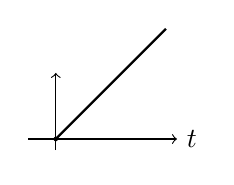
\begin{tikzpicture}[scale=0.7, baseline=(current bounding box.center)]
\draw[->] (-0.5,0) -- (2.2,0) node[right] {$t$};
\draw[->] (0,-0.2) -- (0,1.2) node[above] {};
\draw[thick] (0,0) -- (2,2);
\fill (0,0) circle (1.2pt);
\end{tikzpicture} &
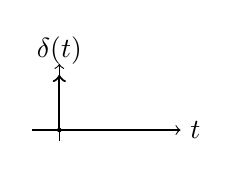
\begin{tikzpicture}[scale=0.7, baseline=(current bounding box.center)]
\draw[->] (-0.5,0) -- (2.2,0) node[right] {$t$};
\draw[->] (0,-0.2) -- (0,1.2) node[above] {};
\draw[->, thick] (0,0) -- (0,1) node[above] {$\delta(t)$};
\fill (0,0) circle (1.2pt);
\end{tikzpicture} \\[15pt]
\multicolumn{3}{c}{单位正弦 $\sin\omega t$} \\[5pt]
\multicolumn{3}{c}{
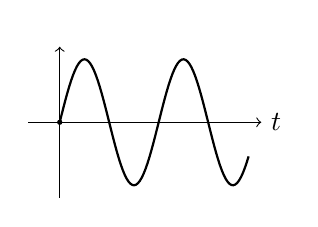
\begin{tikzpicture}[scale=0.8, baseline=(current bounding box.center)]
\draw[->] (-0.5,0) -- (3.2,0) node[right] {$t$};
\draw[->] (0,-1.2) -- (0,1.2) node[above] {};
\draw[domain=0:3, thick, samples=100] plot(\x,{sin(4*\x r)});
\fill (0,0) circle (1.2pt);
\end{tikzpicture}
} \\
\end{tabular}
\end{table}

\begin{itemize}
    \item \textbf{单位阶跃信号}：瞬时阶跃跳变输入，用于考核系统稳态误差与动态响应；
    \item \textbf{单位斜坡信号}：随时间线性增长输入，考核匀速跟踪误差；
    \item \textbf{单位脉冲信号}：单位瞬时冲击信号，用于求解系统单位脉冲响应；
    \item \textbf{单位正弦信号}：周期性交变输入，是频域分析法的基准激励。
\end{itemize}

\section{课程内容导航（全书框架识记）}
本课程整体分为\textbf{系统建模、系统分析、系统综合}三大板块：
\begin{enumerate}
    \item \textbf{控制系统数学建模}：包含微分方程、传递函数、结构图、信号流图四种建模方法；
    \item \textbf{控制系统性能分析}：分为时域分析法、根轨迹分析法、频域分析法；
    \item \textbf{控制系统综合校正（设计）}，细分三条设计路线：
    \begin{itemize}
        \item 基于传递函数+根轨迹法：\textbf{根轨迹校正}；
        \item 基于频率响应法：\textbf{频率域校正}；
        \item 非线性控制系统：采用\textbf{相平面法}分析与校正。
    \end{itemize}
\end{enumerate}

% ===== 恢复全局默认间距（避免影响后续章节）=====
\setlength{\parskip}{0pt plus 1pt}
\setlist{leftmargin=2em, itemsep=0.2em, parsep=0pt}
\renewcommand{\arraystretch}{1}
\setlength{\tabcolsep}{6pt}
% ============================================
% chap02.tex 第二章 控制系统的数学模型（大气排版版）
\chapter{控制系统的数学模型}

% ===== 局部排版优化（仅影响本章，使版面更舒展）=====
\setlength{\parskip}{0.8ex plus 0.3ex minus 0.2ex}   % 段落间距增加
\setlist{
    leftmargin=2.5em,          % 列表左缩进增大
    itemsep=0.6em,             % 条目垂直间距
    parsep=0.3em,              % 条目内段落间距
    topsep=0.8em,              % 列表与上下文间距
    partopsep=0.3em
}
\renewcommand{\arraystretch}{1.5}      % 表格行高增加
\setlength{\tabcolsep}{10pt}           % 表格列间距增加
\addtolength{\abovedisplayskip}{2pt}   % 公式前间距微增
\addtolength{\belowdisplayskip}{2pt}   % 公式后间距微增
% ========================================

\bigskip  % 章节标题后额外留白

\section{本章考核要点}
\begin{enumerate}
    \item 依据物理定律列写系统微分方程的通用步骤；
    \item 机电典型元件微分方程、机电相似性（RC电路$\leftrightarrow$弹簧阻尼质量）；
    \item 微分方程$\leftrightarrow$传递函数$\leftrightarrow$频率特性三者变换关系；
    \item 方块图化简、信号流图+梅森增益公式求总传递函数；
    \item 小信号法非线性系统局部线性化；
    \item 脉冲传递函数（拓展考点）。
\end{enumerate}
\noindent\textbf{补充：}建模两类方法：分析法（已知机理，物理定律）、实验辨识法（机理未知，实测输入输出）；同一物理系统可多模型、不同物理系统可共用同一数学模型（例：RLC二阶电路=弹簧-质量-阻尼二阶系统）。

\medskip

\section{控制系统的时域数学模型——微分方程}
\subsection{微分方程的基本形式}

\paragraph{通用非线性微分方程（全系统通用）}
\[
\begin{split}
a_n \frac{\mathrm{d}^n f_n(y(t))}{\mathrm{d}t^n} &+ a_{n-1} \frac{\mathrm{d}^{n-1} f_{n-1}(y(t))}{\mathrm{d}t^{n-1}} + \dots + a_1 \frac{\mathrm{d} f_1(y(t))}{\mathrm{d}t} + a_0 f_0(y(t)) \\
&= b_m \frac{\mathrm{d}^m g_m(u(t))}{\mathrm{d}t^m} + b_{m-1} \frac{\mathrm{d}^{m-1} g_{m-1}(u(t))}{\mathrm{d}t^{m-1}} + \dots + b_1 \frac{\mathrm{d} g_1(u(t))}{\mathrm{d}t} + b_0 g_0(u(t))
\end{split}
\]
其中 $a_i,b_i$ 为系数，$y(t)$输出，$u(t)$输入，$n\ge m$。

\medskip

\paragraph{线性定常(LTI)标准微分方程（核心公式）}
\[
\begin{split}
a_n \frac{\mathrm{d}^n y(t)}{\mathrm{d}t^n} &+ a_{n-1} \frac{\mathrm{d}^{n-1} y(t)}{\mathrm{d}t^{n-1}} + \dots + a_1 \frac{\mathrm{d}y(t)}{\mathrm{d}t} + a_0 y(t) \\
&= b_m \frac{\mathrm{d}^m u(t)}{\mathrm{d}t^m} + b_{m-1} \frac{\mathrm{d}^{m-1} u(t)}{\mathrm{d}t^{m-1}} + \dots + b_1 \frac{\mathrm{d}u(t)}{\mathrm{d}t} + b_0 u(t)
\end{split}
\]

\medskip

\paragraph{系统分类与判定规则}
\begin{itemize}
    \item \textbf{线性系统：}输入输出全为一次项；\textbf{非线性：}含$y^2,y\dot y$等非线性项
    \item \textbf{定常系统：}全部系数$a_i,b_i$为常数；\textbf{时变：}任意系数含$t$
    \item LTI示例：$\dot y+ay=u$；LTV示例：$\dot y+a(t)y=bu$
    \item NLTI示例：$\dot y-y^2=bu$；NLTV示例：$\dot y-y^2=b(t)u$
\end{itemize}

\subsection{建立微分方程（建模三步必考）}
\begin{enumerate}
    \item 列元件物理方程；\item 消去中间变量；\item 输出导数放左侧、输入导数放右侧，降幂整理。
\end{enumerate}

\paragraph{电路建模（KVL/KCL）}
RLC串联：输入$u_i$、输出$u_o=u_C$
\[
LC\frac{\mathrm{d}^2 u_o}{\mathrm{d}t^2}+RC\frac{\mathrm{d}u_o}{\mathrm{d}t}+u_o=u_i(t)
\]

\medskip

\paragraph{机械元件与建模}
\begin{table}[htbp]
\centering
\caption{机械元件基本方程}
\begin{tabular}{ll}
\toprule
元件 & 方程 \\
\midrule
质量 & $F=m\ddot x$ \\
弹簧 & $F=k(x_1-x_2)$ \\
阻尼 & $F=f(\dot x_1-\dot x_2)$ \\
转动惯量 & $T=J\ddot\theta$ \\
\bottomrule
\end{tabular}
\end{table}

弹簧-质量-阻尼（外力$F$，位移$y$）：
\[
m\ddot y+f\dot y+ky=F(t)
\]
\noindent\textbf{机电相似：} RLC与弹簧阻尼质量同型二阶方程。

\subsection{线性系统的性质}
\[
x=ax_1+bx_2 \quad\Longrightarrow\quad y=ay_1+by_2
\]

\subsection{非线性系统的线性化（小信号法，必考）}
平衡点$x_0$泰勒展开，略去高阶小量：
\[
\Delta y=\left.\frac{\mathrm{d}f}{\mathrm{d}x}\right|_{x_0}\cdot\Delta x,\quad K=\left.\frac{\mathrm{d}f}{\mathrm{d}x}\right|_{x_0}
\]
\textbf{不可线性化：}继电器、死区、间隙等本质非线性。

\bigskip

\section{控制系统的复域数学模型——传递函数}
\subsection{拉普拉斯变换定义}
\[
F(s)=\mathcal{L}[f(t)]=\int_0^\infty f(t)e^{-st}\mathrm{d}t
\]

\paragraph{常用变换对（必背）}
\begin{table}[htbp]
\centering
\caption{常见拉普拉斯变换对}
\begin{tabular}{ccc}
\toprule
$f(t)$ & $F(s)$ & 条件 \\
\midrule
$\delta(t)$ & $1$ & \\
$1(t)$ & $\dfrac1s$ & \\
$t$ & $\dfrac1{s^2}$ & \\
$\dfrac{t^{n-1}}{(n-1)!}$ & $\dfrac1{s^n}$ & $n=1,2,\dots$ \\
$e^{-at}$ & $\dfrac1{s+a}$ & \\
$\sin\omega t$ & $\dfrac{\omega}{s^2+\omega^2}$ & \\
$\cos\omega t$ & $\dfrac{s}{s^2+\omega^2}$ & \\
$\dfrac{t^{n-1}}{(n-1)!}e^{-at}$ & $\dfrac1{(s+a)^n}$ & $n=1,2,\dots$ \\
\bottomrule
\end{tabular}
\end{table}

\paragraph{拉普拉斯变换性质}
\begin{enumerate}
\item \textbf{线性性质：}$\mathcal{L}[a f_1(t)+b f_2(t)]=aF_1(s)+bF_2(s)$

\item \textbf{微分性质：}
一阶：$\displaystyle \mathcal{L}\left[\frac{\mathrm{d}f(t)}{\mathrm{d}t}\right]=sF(s)-f(0)$
$n$阶：$\displaystyle \mathcal{L}\left[\frac{\mathrm{d}^n f(t)}{\mathrm{d}t^n}\right]=s^nF(s)-s^{n-1}f(0)-\dots-f^{(n-1)}(0)$
零初值：$\mathcal{L}[f^{(n)}(t)]=s^nF(s)$

\item \textbf{积分性质：}
单次积分：$\displaystyle \mathcal{L}\left[\int f(t)\mathrm{d}t\right]=\frac1sF(s)+\frac1s f(0)$
$n$重积分零初值：$\displaystyle \mathcal{L}\left[\underbrace{\int\dots\int}_{n} f(t)\mathrm{d}t^n\right]=\frac1{s^n}F(s)$

\item \textbf{初值定理：}$\displaystyle \lim_{t\to0^+}f(t)=\lim_{s\to\infty}sF(s)$

\item \textbf{终值定理：}$\displaystyle \lim_{t\to\infty}f(t)=\lim_{s\to0}sF(s)$（$sF(s)$极点全在左半平面）

\item \textbf{位移定理：}
时域延迟：$\mathcal{L}\big[f(t-\tau_0)\big]=e^{-\tau_0 s}F(s)$
复频位移：$\mathcal{L}\big[e^{-at}f(t)\big]=F(s+a)$
\end{enumerate}

其他常用性质：
\[
\begin{aligned}
&\mathcal{L}\big[f(t-a)\cdot 1(t-a)\big]=e^{-as}F(s)\quad(a>0),\\
&\mathcal{L}\big[t f(t)\big]=-\frac{\mathrm{d}F(s)}{\mathrm{d}s},\\
&\mathcal{L}\big[\tfrac1t f(t)\big]=\int_s^\infty F(s)\mathrm{d}s,\\
&\mathcal{L}\big[f(\tfrac ta)\big]=aF(as)\quad(a>0).
\end{aligned}
\]

\medskip

\paragraph{留数定理（拉普拉斯逆变换）}
若$F(s)$为有理分式，极点$s=p_i\;(i=1,2,\dots,k)$，则
\[
f(t)=\mathcal{L}^{-1}[F(s)]=\frac1{2\pi j}\int_{\sigma-j\infty}^{\sigma+j\infty}F(s)e^{st}\mathrm{d}s=\sum_{i=1}^k \mathrm{Res}\big[F(s)e^{st},\,s=p_i\big],\quad t>0
\]
\begin{itemize}
    \item \textbf{一阶极点 $s=p$：}$\displaystyle \mathrm{Res}\big[F(s)e^{st},p\big]=\lim_{s\to p}(s-p)F(s)e^{st}$
    \item \textbf{$r$阶重极点 $s=p$：}$\displaystyle \mathrm{Res}=\frac1{(r-1)!}\lim_{s\to p}\frac{\mathrm{d}^{r-1}}{\mathrm{d}s^{r-1}}\big[(s-p)^r F(s)e^{st}\big]$
\end{itemize}

\subsection{传递函数的概念与说明}
\paragraph{定义（零初始条件下）}
系统输出量的拉氏变换与输入量的拉氏变换之比：
\[
G(s) = \frac{Y(s)}{R(s)} = \frac{b_m s^m + b_{m-1} s^{m-1} + \dots + b_1 s + b_0}{a_n s^n + a_{n-1} s^{n-1} + \dots + a_1 s + a_0}
\]

\paragraph{传递函数的八点详细说明}
\begin{enumerate}
    \item 它是复域数学模型，和系统微分方程一一对应；
    \item 只取决于系统或元件的结构和参数，与系统输入信号无关；
    \item 形式与输入、输出信号的选取位置密切相关；
    \item 分子分母是$s$的降幂有理多项式，系数均为实数，零点、极点只可为实数或共轭复数；
    \item 物理可实现系统分母阶次大于或等于分子阶次（$n\ge m$）；
    \item 无法直接反映系统及元件的物理结构；
    \item 令分母多项式等于零，可得到系统的特征方程；
    \item 传递函数和系统单位脉冲响应互为拉普拉斯变换对。
\end{enumerate}

\paragraph{传递函数的局限性}
\begin{enumerate}
    \item 原则上不反映非零初始条件时系统响应的全部信息；
    \item 适合用于描述单输入单输出（SISO）系统；
    \item 只能用于表示线性定常系统。
\end{enumerate}

\medskip

\paragraph{零初始条件说明（考试常考点）}
\begin{itemize}
    \item 输入量在 $t\ge0$ 作用于系统，$t=0^-$ 时输入及其各阶导数均为零；
    \item 输入加入前系统处于稳定工作状态，$t=0^-$ 时输出及其各阶导数也为零。
\end{itemize}

\medskip

\paragraph{由微分方程推导传递函数}
对线性定常系统微分方程：
\[
a_n y^{(n)}(t) + a_{n-1} y^{(n-1)}(t) + \dots + a_1 \dot{y}(t) + a_0 y(t) = b_m r^{(m)}(t) + \dots + b_1 \dot{r}(t) + b_0 r(t)
\]
零初始条件下，取拉普拉斯变换：
\[
(a_n s^n + a_{n-1} s^{n-1} + \dots + a_1 s + a_0)Y(s) = (b_m s^m + \dots + b_1 s + b_0)R(s)
\]
整理即得传递函数表达式。

\medskip

\paragraph{传递函数的三种标准形式（必考）}
\subparagraph{1. 零、极点形式（根轨迹分析常用）}
将传递函数因式分解，写成零极点乘积形式：
\[
G(s) = \frac{Y(s)}{R(s)} = \frac{b_m s^m + b_{m-1} s^{m-1} + \dots + b_1 s + b_0}{a_n s^n + a_{n-1} s^{n-1} + \dots + a_1 s + a_0}
\]
\[
G(s) = \frac{b_0}{a_0} \cdot \frac{(s-z_1)(s-z_2)\cdots(s-z_m)}{(s-p_1)(s-p_2)\cdots(s-p_n)} = K^* \cdot \frac{\prod_{i=1}^m (s-z_i)}{\prod_{j=1}^n (s-p_j)}
\]
其中：
\begin{itemize}
    \item 零点：$z_i\;(i=1,2,\dots,m)$，使分子为零的复频率；
    \item 极点：$p_j\;(j=1,2,\dots,n)$，使分母为零的复频率，也是微分方程的特征根；
    \item 根轨迹增益（传递系数）：$K^* = \dfrac{b_0}{a_0}$。
\end{itemize}

\subparagraph{2. 时间常数形式（频率法分析常用）}
将传递函数整理为以“时间常数”为系数的标准形式，方便绘制频率特性：
\[
G(s) = \frac{b_m}{a_n} \cdot \frac{(\tau_1 s+1)(\tau_2^2 s^2 + 2\zeta\tau_2 s + 1)\cdots(\tau_i s+1)}{(T_1 s+1)(T_2^2 s^2 + 2\zeta T_2 s + 1)\cdots(T_j s+1)}
\]
其中：
\begin{itemize}
    \item 一次因子 $(\tau_i s+1)$ 对应实数零极点；
    \item 二次因子 $(T_j^2 s^2 + 2\zeta T_j s + 1)$ 对应共轭复数零极点；
    \item 时间常数：$\tau_i$（分子）和 $T_j$（分母）；
    \item 传递系数（静态增益）：$K = \dfrac{b_m}{a_n}$。
\end{itemize}

\subparagraph{3. 两种形式的转换关系}
从零极点形式到时间常数形式的转换，需要将零极点因子改写为“一次项+常数”的形式：
\[
G(s) = K^* \cdot \frac{\prod_{i=1}^m (s-z_i)}{\prod_{j=1}^n (s-p_j)} = K^* \cdot \frac{\left( \prod_{i=1}^m \frac{1}{-z_i} \right) \prod_{i=1}^m \left( \frac{1}{-z_i} s + 1 \right)}{\left( \prod_{j=1}^n \frac{1}{-p_j} \right) \prod_{j=1}^n \left( \frac{1}{-p_j} s + 1 \right)}
\]
两种增益的关系为：
\[
K = K^* \cdot \frac{\prod_{i=1}^m (-z_i)}{\prod_{j=1}^n (-p_j)}
\]

\subsection{典型环节的传递函数（8类全细化，必考）}
控制系统复杂传递函数都可拆解为以下基础环节的组合：
\begin{enumerate}
    \item \textbf{放大环节（比例环节）}
    时域关系：$y(t)=Kr(t)$，传递函数：$\displaystyle G(s)=\frac{Y(s)}{R(s)}=K$，几乎所有控制系统都包含该环节。

    \item \textbf{惯性环节}
    微分方程：$\displaystyle T\frac{\mathrm{d}y(t)}{\mathrm{d}t}+y(t)=r(t)$，传递函数：$\displaystyle G(s)=\frac{Y(s)}{R(s)}=\frac1{Ts+1}$，$T$为时间常数；$T=0$时退化为放大环节。

    \item \textbf{积分环节}
    微分方程：$\displaystyle y(t)=\int r(t)\mathrm{d}t$，传递函数：$\displaystyle G(s)=\frac{Y(s)}{R(s)}=\frac1s$，输出为输入对时间的积分。

    \item \textbf{震荡环节}（$0\le\zeta<1$）
    微分方程：$\displaystyle T^2\frac{\mathrm{d}^2y(t)}{\mathrm{d}t^2}+2\zeta T\frac{\mathrm{d}y(t)}{\mathrm{d}t}+y(t)=r(t)$，
    传递函数：$\displaystyle G(s)=\frac{Y(s)}{R(s)}=\frac{\omega_n^2}{s^2+2\zeta\omega_n s+\omega_n^2}$。

    \item \textbf{纯微分环节}
    微分方程：$\displaystyle y(t)=\frac{\mathrm{d}r(t)}{\mathrm{d}t}$，传递函数：$\displaystyle G(s)=\frac{Y(s)}{R(s)}=s$，输出为输入对时间的微分。

    \item \textbf{一阶微分环节}
    微分方程：$\displaystyle y(t)=\tau\frac{\mathrm{d}r(t)}{\mathrm{d}t}+r(t)$，传递函数：$\displaystyle G(s)=\frac{Y(s)}{R(s)}=\tau s+1$。

    \item \textbf{二阶微分环节}
    微分方程：$\displaystyle y(t)=\tau^2\frac{\mathrm{d}^2r(t)}{\mathrm{d}t^2}+2\zeta\tau\frac{\mathrm{d}r(t)}{\mathrm{d}t}+r(t)$，
    传递函数：$\displaystyle G(s)=\frac{Y(s)}{R(s)}=\tau^2 s^2+2\zeta\tau s+1$。

    \item \textbf{延迟环节}
    微分方程：$y(t)=r(t-\tau)$，传递函数：$\displaystyle G(s)=\frac{Y(s)}{R(s)}=e^{-\tau s}$，$\tau$为延迟时长。
\end{enumerate}

\bigskip

\section{控制系统的方框图和信号流图}
\subsection{2.3.1 方框图的概念和绘制}
方框图是用图形直观描述系统各元件信号传递关系的数学模型，能清晰展示信号流向、环节连接方式与系统结构，方便求解复杂系统传递函数。

对于结构复杂的多回路系统，单纯利用方框图化简方法求取系统整体传递函数，计算过程会变得十分繁琐困难。

\subsection{2.3.2 方框图化简}
\begin{enumerate}
    \item \textbf{串联环节等效}：总传递函数 $G(s) = G_1(s)G_2(s)$；
    \item \textbf{并联环节等效}：总传递函数 $G(s) = G_1(s) + G_2(s)$；
    \item \textbf{反馈闭环等效}：负反馈 $\displaystyle \Phi(s) = \frac{G(s)}{1 + G(s)H(s)}$，正反馈分母改为 $1-G(s)H(s)$。
\end{enumerate}

\subsection{2.3.3 信号流图的概念和绘制}
信号流图是表示系统中各变量间相互关系以及信号传递的另一种图解方法。
\begin{itemize}
    \item 节点：表示系统的变量；
    \item 支路：相当于乘法器，信号流经支路时，被乘以支路增益而变换为另一信号；
    \item 信号在支路上只能沿箭头单向传递；
    \item 系统节点变量的设置不唯一，因此同一个系统的信号流图不是唯一的。
\end{itemize}

\paragraph{节点运算规则}
节点同时具备两种作用：
\begin{enumerate}
    \item 对所有来自流入支路的信号作加法运算；
    \item 将流入信号之和，传输给所有流出支路。
\end{enumerate}
\[
\begin{cases}
w = au+bv \\
x = cw = c(au+bv) \\
y = dw = d(au+bv)
\end{cases}
\]

\paragraph{信号流图核心术语}
\begin{itemize}
    \item \textbf{源节点（输入节点）}：只有信号输出，无信号输入；
    \item \textbf{阱节点（输出节点）}：只有信号输入，无信号输出；
    \item \textbf{混合节点}：既有输入支路，又有输出支路；
    \item \textbf{前向通路}：信号从输入节点至输出节点传递，每个节点只通过1次的通路；
    \item \textbf{单独回路}：起点和终点为同一节点，信号遍历节点不重复的闭合通路；
    \item \textbf{回路增益}：回路中所有支路增益的乘积；
    \item \textbf{不接触回路}：多个回路之间没有任何公共节点，反之称为接触回路。
\end{itemize}

\paragraph{方框图 $\leftrightarrow$ 信号流图对应转换规则}
方框图单元 $\rightarrow$ 信号流图单元：
输入相加点 $\rightarrow$ 混合节点；引出点 $\rightarrow$ 混合节点；方框环节 $\rightarrow$ 增益支路；信号连线 $\rightarrow$ 有向支路。

\subsection{2.3.4 梅森增益公式}
复杂系统无需化简框图，可直接通过梅森公式求解系统总传递函数，公式为：
\[
P = \frac{1}{\Delta} \sum_{k=1}^n P_k \Delta_k
\]

\paragraph{参数定义}
\begin{itemize}
    \item $P$：系统总传输增益（闭环总传递函数）；
    \item $P_k$：第 $k$ 条前向通路的通路总增益；
    \item $\Delta$：信号流图特征式
    \[
    \Delta = 1 - \sum L_a + \sum L_b L_c - \sum L_d L_e L_f + \dots
    \]
    \begin{itemize}
        \item $\sum L_a$：所有单独回路增益之和；
        \item $\sum L_b L_c$：每两个互不接触回路增益乘积之和；
        \item $\sum L_d L_e L_f$：每三个互不接触回路增益乘积之和；
    \end{itemize}
    \item $\Delta_k$：第 $k$ 条前向通路的余子式
    \begin{itemize}
        \item 若通路与所有回路都接触：$\boldsymbol{\Delta_k=1}$；
        \item 若通路与所有回路都不接触：$\boldsymbol{\Delta_k=\Delta}$；
    \end{itemize}
\end{itemize}

\bigskip

\section{第2章 小结}
\subsection{经典控制理论的数学模型体系}
经典控制理论中常用的控制系统数学模型包含四类：
\begin{itemize}
    \item 微分方程（时域最原始模型）
    \item 传递函数（复域核心模型）
    \item 方框图（图形化模块模型）
    \item 信号流图（简化图形化模型，适配梅森公式）
\end{itemize}

\subsection{系统分析与综合的闭环逻辑}
由数学模型得到系统模型后，可开展双向工作：
\begin{enumerate}
    \item \textbf{系统分析（正向推导）}：由系统模型计算控制系统的各项性能指标，判断其是否满足设计要求，分为三类方法：
    \begin{itemize}
        \item 时域法
        \item 复域法
        \item 频域法
    \end{itemize}
    \item \textbf{系统综合（反向设计）}：根据性能指标要求，寻求改进系统性能、使其满足设计规范的校正方法，形成闭环优化流程。
\end{enumerate}

% ===== 恢复全局默认间距（避免影响后续章节）=====
\setlength{\parskip}{0pt plus 1pt}
\setlist{leftmargin=2em, itemsep=0.2em, parsep=0pt}
\renewcommand{\arraystretch}{1}
\setlength{\tabcolsep}{6pt}
% ============================================
% chap03.tex 第三章 控制系统的时域分析（大气排版版）
\chapter{控制系统的时域分析}

% ===== 局部排版优化（仅影响本章，使版面更舒展）=====
\setlength{\parskip}{0.8ex plus 0.3ex minus 0.2ex}   % 段落间距增加
\setlist{
    leftmargin=2.5em,          % 列表左缩进增大
    itemsep=0.6em,             % 条目垂直间距
    parsep=0.3em,              % 条目内段落间距
    topsep=0.8em,              % 列表与上下文间距
    partopsep=0.3em
}
\renewcommand{\arraystretch}{1.5}      % 表格行高增加
\setlength{\tabcolsep}{10pt}           % 表格列间距增加
\addtolength{\abovedisplayskip}{2pt}   % 公式前间距微增
\addtolength{\belowdisplayskip}{2pt}   % 公式后间距微增
% ========================================

\bigskip  % 章节标题后额外留白

\section{本章考核要点}
\begin{enumerate}
    \item 典型输入信号与时域响应分类（动态/稳态）；
    \item 一阶、二阶系统的单位阶跃响应与时域性能指标计算；
    \item 高阶系统的主导极点简化方法；
    \item 劳斯判据稳定性分析；
    \item 稳态误差计算（静态误差系数法、终值定理法）。
\end{enumerate}
\noindent\textbf{补充：}时域法是最基本的分析方法，是复域法、频域法的基础，直接在时间域对系统进行分析和设计，直观准确，但求解解析解过程较繁琐。

\medskip

\section{系统时间响应与性能指标概述}
\subsection{课程任务与体系结构}
控制系统的分析与综合构成闭环逻辑：
\begin{enumerate}
    \item \textbf{系统分析}：由系统模型计算控制系统的各项性能指标，判断其是否满足设计要求，包括时域法、复域法、频域法三类方法；
    \item \textbf{系统综合}：根据性能指标要求，寻求改进系统性能、使其满足设计规范的校正方法。
\end{enumerate}

\subsection{本章主要内容}
\begin{enumerate}
    \item 3.1 系统时间响应的性能指标；
    \item 3.2 一阶系统的时域分析；
    \item 3.3 二阶系统的时域分析；
    \item 3.4 高阶系统的时域分析；
    \item 3.5 线性系统的稳定性分析；
    \item 3.6 线性系统的稳态误差计算。
\end{enumerate}

\subsection{系统时间响应的求解步骤}
分析系统性能的通用步骤：
\begin{enumerate}
    \item 给出控制系统的闭环传递函数 $\Phi(s)$；
    \item 用 $Y(s) = \Phi(s)R(s)$ 求出系统输出的拉氏变换 $Y(s)$，再通过拉普拉斯逆变换求 $y(t)$；
    \item 根据 $y(t)$ 分析系统动态与稳态性能；
    \item 建立系统性能与传递函数参数之间的对应关系。
\end{enumerate}
\[
\text{数学模型} \xrightarrow{\text{典型输入下求解微分方程}} \text{时域响应} \rightarrow \text{性能指标}
\]

\subsection{典型输入信号}
控制系统常用的典型测试信号，用于统一标准下的性能对比：
\begin{table}[htbp]
\centering
\caption{典型输入信号及其拉普拉斯变换}
\begin{tabular}{ccccc}
\toprule
信号名称 & 时域表达式 $f(t)$ & 拉氏变换 $F(s)$ & 典型应用场景 \\
\midrule
单位脉冲 & $\delta(t)$ & $1$ & 冲击信号、电脉冲测试 \\
单位阶跃 & $1(t) = \begin{cases} 1, & t\ge0 \\ 0, & t<0 \end{cases}$ & $\dfrac{1}{s}$ & 开关量、阶跃扰动测试 \\
单位斜坡 & $t\cdot1(t) = \begin{cases} t, & t\ge0 \\ 0, & t<0 \end{cases}$ & $\dfrac{1}{s^2}$ & 等速跟踪、恒速输入测试 \\
单位加速度 & $\dfrac{t^2}{2}\cdot1(t) = \begin{cases} t^2/2, & t\ge0 \\ 0, & t<0 \end{cases}$ & $\dfrac{1}{s^3}$ & 恒加速跟踪测试 \\
\bottomrule
\end{tabular}
\end{table}
信号之间的时域关系：单位阶跃是单位脉冲的积分，单位斜坡是单位阶跃的积分，单位加速度是单位斜坡的积分，对应复域关系为乘以 $1/s$。

\subsection{动态过程与稳态过程}
系统响应按时间阶段分为两类：
\begin{enumerate}
    \item \textbf{动态过程（过渡过程/瞬态过程）}：典型输入作用下，系统输出从初始状态到最终状态的响应过程。稳定系统的动态过程是收敛的，不稳定系统的动态过程是发散或等幅振荡的。
    \item \textbf{稳态过程（稳态响应）}：典型输入作用下，当 $t\to\infty$ 时的系统输出，表征系统输出最终复现输入量的程度，用稳态性能指标描述。
\end{enumerate}

\subsection{动态性能与稳态性能}
控制系统的基本性能要求可概括为“稳、准、快”：
\begin{itemize}
    \item \textbf{稳（稳定性）}：系统受扰动影响后能回到原来的平衡位置，是系统正常工作的基本前提；
    \item \textbf{准（稳态性能）}：稳态输出与理想输出之间的误差（稳态误差）要小，反映系统的控制精度；
    \item \textbf{快（动态性能）}：阶跃响应的过渡过程要平稳、迅速，反映系统的动态响应速度与平稳性。
\end{itemize}
稳态误差是描述系统稳态性能的核心指标，通常在阶跃、斜坡或加速度信号作用下计算。若 $t\to\infty$ 时系统输出不等于输入或输入的确定函数，则存在稳态误差，其大小反映了系统的控制精度和抗扰动能力。

\subsection{线性系统时域性能指标（单位阶跃响应）}
仅对稳定系统定义以下时域性能指标：
\begin{itemize}
    \item \textbf{延迟时间 $t_d$}：阶跃响应第一次达到终值的 $50\%$ 所需的时间；
    \item \textbf{上升时间 $t_r$}：阶跃响应从终值的 $10\%$ 上升到终值的 $90\%$ 所需的时间；有振荡时，也可定义为从 $0$ 到第一次达到终值所需的时间；
    \item \textbf{峰值时间 $t_p$}：阶跃响应越过终值达到第一个峰值所需的时间；
    \item \textbf{超调量 $\sigma\%$}：峰值超出终值的百分比：
    \[
    \sigma\% = \frac{y(t_p) - y(\infty)}{y(\infty)} \times 100\%
    \]
    \item \textbf{调节时间 $t_s$}：阶跃响应到达并保持在终值的 $5\%$ 或 $2\%$ 误差带内所需的最短时间，满足 $|y(t)-y(\infty)| \le \Delta y(\infty),\ t\le t_s$；
    \item \textbf{振荡次数 $N$}：在 $t\le t_s$ 时间内，单位阶跃响应穿越稳态值 $y(\infty)$ 次数的一半。
\end{itemize}

\bigskip

\section{一阶系统的时域分析}
一阶系统标准闭环传递函数：
\[
\Phi(s)=\frac{C(s)}{R(s)}=\frac{1}{Ts+1}
\]
$T$ 为一阶系统的时间常数，直接决定系统动态响应速度与稳态跟踪能力。

\subsection{一阶系统单位阶跃响应回顾}
输入为单位阶跃信号 $R(s)=\frac{1}{s}$，输出：
\[
Y(s)=\frac{1}{Ts+1}\cdot\frac{1}{s}
\]
拉氏反变换得时域响应：
\[
y(t)=1-e^{-\frac{t}{T}},\quad t\ge 0
\]
关键特征：$y(T)=0.632$、$y(2T)=0.865$、$y(3T)=0.95$、$y(4T)=0.98$；\textbf{时间常数 $T$ 越小，响应上升速度越快，调节时间越短}。

思考：4条阶跃响应曲线时间常数分别为 $0.5,1,2,5$，曲线上升速度从快到慢对应 $T=0.5>1>2>5$，最陡曲线对应 $T=0.5$，最平缓曲线对应 $T=5$。

\subsection{一阶系统单位脉冲响应}
输入为单位脉冲信号 $r(t)=\delta(t),\ R(s)=1$，输出：
\[
Y(s)=\frac{1}{Ts+1}
\]
拉氏反变换得：
\[
y(t)=\frac{1}{T}e^{-\frac{t}{T}},\quad t\ge 0
\]
关键特征参数：
\[
\begin{cases}
y(0)=\displaystyle\frac{1}{T}\\
y(\infty)=0\\
y'(0)=-\displaystyle\frac{1}{T^2}\\
y(T)=\displaystyle\frac{0.368}{T}
\end{cases}
\]
响应特点：
\begin{enumerate}
    \item $y(t)$ 是单调连续下降的指数曲线；
    \item 终值为 $0$，脉冲输入下稳态误差为 $0$；
    \item 动态性能完全由时间常数 $T$ 决定；
    \item 脉冲响应做拉氏变换可直接得到系统传递函数，完整表征系统特性。
\end{enumerate}

\subsection{一阶系统单位斜坡响应}
输入为单位斜坡信号 $r(t)=t,\ R(s)=\frac{1}{s^2}$，输出：
\[
Y(s)=\frac{1}{Ts+1}\cdot\frac{1}{s^2}
\]
拉氏反变换得：
\[
y(t)=t-T\left(1-e^{-\frac{t}{T}}\right),\quad t\ge 0
\]
响应特点：
\begin{enumerate}
    \item $t\to\infty$ 时，$y(t)\to t-T$；
    \item 跟踪斜坡信号存在稳态误差，稳态误差数值等于时间常数 $T$；
    \item 减小 $T$ 既能加快响应速度，也能减小斜坡跟踪的稳态误差。
\end{enumerate}

\subsection{一阶系统单位匀加速度响应}
输入为单位匀加速度信号 $r(t)=\frac12 t^2,\ R(s)=\frac{1}{s^3}$，输出：
\[
Y(s)=\frac{1}{Ts+1}\cdot\frac{1}{s^3}
\]
拉氏反变换得：
\[
y(t)=\frac12 t^2-Tt+T^2\left(1-e^{-\frac{t}{T}}\right),\quad t\ge 0
\]
响应特点：
\begin{enumerate}
    \item 跟踪误差会随时间推移持续增大；
    \item 一阶系统无法实现对匀加速度信号的有效跟踪。
\end{enumerate}

\subsection{一阶系统时域分析小结}
\begin{table}[htbp]
\centering
\caption{一阶系统对典型输入信号的响应汇总}
\begin{tabular}{ccccc}
\toprule
输入 $r(t)$ & $R(s)$ & $C(s)=\Phi(s)R(s)$ & 时域响应 $c(t)$ \\
\midrule
$\delta(t)$ & $1$ & $\displaystyle\frac{1}{Ts+1}$ & $\displaystyle k(t)=\frac{1}{T}e^{-\frac{t}{T}}$ \\
$1(t)$ & $\displaystyle\frac{1}{s}$ & $\displaystyle\frac{1}{s}-\frac{1}{s+\frac{1}{T}}$ & $\displaystyle h(t)=1-e^{-\frac{t}{T}}$ \\
$t$ & $\displaystyle\frac{1}{s^2}$ & $\displaystyle\frac{1}{s^2}-\frac{T}{s}+\frac{T}{s+\frac{1}{T}}$ & $\displaystyle c(t)=t-T\left(1-e^{-\frac{t}{T}}\right)$ \\
$\frac12 t^2$ & $\displaystyle\frac{1}{s^3}$ & / & $\displaystyle c(t)=\frac12 t^2-Tt+T^2\left(1-e^{-\frac{t}{T}}\right)$ \\
\bottomrule
\end{tabular}
\end{table}
\begin{enumerate}
    \item \textbf{等价关系}：系统对输入导数的响应 = 对原输入响应的导数；系统对输入积分的响应 = 对原输入响应的积分；
    \item \textbf{动态特性}：时间常数 $T$ 越大，响应速度越慢、调节时间越长，反之响应越快；
    \item \textbf{跟踪能力}：阶跃输入无稳态误差；斜坡输入稳态误差等于 $T$；加速度输入稳态误差趋于无穷，无法跟踪。
\end{enumerate}

\bigskip

\section{二阶系统的时域分析}
\subsection{二阶系统的数学模型}
\subsubsection{标准形式定义}
标准二阶系统微分方程：
\[
\ddot{y}+2\zeta\omega_n \dot{y}+\omega_n^2 y=\omega_n^2 r
\]
闭环传递函数（首1标准型）：
\[
\Phi(s)=\frac{C(s)}{R(s)}=\frac{\omega_n^2}{s^2+2\zeta\omega_n s+\omega_n^2}
\]
尾1标准型闭环传递函数：
\[
\Phi(s)=\frac{1}{T^2 s^2+2T\zeta s+1}
\]
其中：
\begin{itemize}
    \item $\omega_n$：自然频率（或无阻尼振荡频率）；
    \item $\zeta$：阻尼比（或阻尼系数）。
\end{itemize}

单位反馈结构对应的开环传递函数：
\[
G(s)=\frac{\omega_n^2}{s(s+2\zeta\omega_n)}
\]

\subsubsection{电动伺服系统实例}
以电动伺服机构为例，通过电位计测偏差、放大器放大、直流电机驱动负载，可推导出上述标准二阶形式，完整框图可通过环节串联与反馈化简得到标准闭环表达式。

\subsubsection{非标准二阶系统标准化方法}
若已知单位反馈开环传函 $G(s)=\dfrac{K}{s(Ts+1)}$，变形拆分：
\[
G(s)=\frac{K/T}{s\left(s+\frac1T\right)}
\]
联立标准形式参数对应方程组：
\[
\begin{cases}
\omega_n^2=\displaystyle\frac{K}{T}\\[4pt]
2\zeta\omega_n=\displaystyle\frac1T
\end{cases}
\]
求解得：
\[
\begin{cases}
\omega_n=\sqrt{\displaystyle\frac{K}{T}}\\[4pt]
\zeta=\sqrt{\displaystyle\frac{1}{4TK}}
\end{cases}
\]
反向换算关系：
\[
\frac{K}{T}=\omega_n^2,\quad TK=\frac{1}{4\zeta^2}
\]

\subsubsection{标准二阶系统特征方程与特征根}
特征方程：
\[
s^2+2\zeta\omega_n s+\omega_n^2=0
\]
求解特征根：
\[
s_{1,2}=-\zeta\omega_n\pm\omega_n\sqrt{\zeta^2-1}
\]
阻尼比 $\zeta$ 的取值直接决定特征根在 $s$ 平面上的位置，分区间讨论：
\begin{enumerate}
    \item $\boldsymbol{\zeta>0}$，根实部为负（系统稳定）：
    \begin{itemize}
        \item $0<\zeta<1$：一对共轭复根（欠阻尼）；
        \item $\zeta=1$：一对相等实根（临界阻尼）；
        \item $\zeta>1$：一对不等实根（过阻尼）。
    \end{itemize}
    \item $\boldsymbol{\zeta=0}$，实部为0：纯虚共轭根 $s_{1,2}=\pm j\omega_n$（无阻尼，等幅振荡）；
    \item $\boldsymbol{\zeta<0}$，根实部为正（系统不稳定）：
    \begin{itemize}
        \item $-1<\zeta<0$：一对共轭复根（负阻尼，发散振荡）；
        \item $\zeta=-1$：一对相等正实根；
        \item $\zeta<-1$：一对不等正实根。
    \end{itemize}
\end{enumerate}

阻尼工况分类汇总：
\begin{itemize}
    \item $0<\zeta<1$：欠阻尼；
    \item $\zeta=1$：临界阻尼；
    \item $\zeta>1$：过阻尼；
    \item $\zeta=0$：无阻尼；
    \item $-1<\zeta<0$：负阻尼。
\end{itemize}

\subsection{二阶系统的单位阶跃响应}
\subsubsection{① 欠阻尼 $\boldsymbol{0<\zeta<1}$ 的情况}
共轭复数极点：
\[
s_{1,2}=-\zeta\omega_n\pm j\omega_n\sqrt{1-\zeta^2}
\]
定义有阻尼振荡频率：
\[
\omega_d=\omega_n\sqrt{1-\zeta^2}
\]

时域完整表达式：
\[
y(t)=1-e^{-\zeta\omega_n t}\left(\cos\omega_d t+\frac{\zeta}{\sqrt{1-\zeta^2}}\sin\omega_d t\right),\quad t\ge0
\]
等价合并正弦相位形式：
\[
y(t)=1-\frac{e^{-\zeta\omega_n t}}{\sqrt{1-\zeta^2}}\sin\left(\omega_d t+\theta\right),\quad t\ge0
\]
其中相位角：
\[
\theta=\arctan\frac{\sqrt{1-\zeta^2}}{\zeta}=\arccos\zeta
\]

将响应拆分为稳态分量、暂态分量：
\[
y(t)=\underbrace{1}_{\text{稳态分量}}-\underbrace{\frac{e^{-\zeta\omega_n t}}{\sqrt{1-\zeta^2}}\sin\left(\omega_d t+\theta\right)}_{\text{暂态分量}}
\]
响应包络线约束：$\displaystyle 1\pm \frac{e^{-\zeta\omega_n t}}{\sqrt{1-\zeta^2}}$。

\paragraph{欠阻尼单位阶跃响应特点}
\begin{enumerate}
    \item 暂态分量是衰减的正弦振荡；
    \item 暂态分量的衰减速度取决于衰减系数 $\zeta\omega_n$；
    \item 系统输出稳态值恒为 $1$；
    \item 阶跃信号作用下不存在稳态误差；
    \item 响应曲线被包络线约束，呈衰减振荡收敛至稳态。
\end{enumerate}

\subsubsection{② 无阻尼 $\boldsymbol{\zeta=0}$ 的情况}
闭环极点：
\[
s_{1,2}=\pm j\omega_n
\]
极点落在虚轴上，代入通用阶跃响应公式，$\zeta=0,\theta=90^\circ$：
\[
y(t)=1-\cos\left(\omega_n t\right),\quad t\ge0
\]

\paragraph{无阻尼响应特点}
\begin{enumerate}
    \item 单位阶跃响应为等幅振荡过程；
    \item 超调量 $\sigma_p=100\%$，调节时间 $t_s\to\infty$；
    \item 系统临界稳定，无法正常工作。
\end{enumerate}

\subsubsection{③ 临界阻尼 $\boldsymbol{\zeta=1}$ 的情况}
一对相同负实数极点：
\[
s_{1,2}=-\omega_n
\]
单位阶跃响应：
\[
y(t)=1-e^{-\omega_n t}\left(1+\omega_n t\right),\quad t\ge0
\]

求导：$\displaystyle \frac{dy(t)}{dt}=\omega_n^2 t e^{-\omega_n t}$，$t=0$ 时曲线斜率为 $0$。

\paragraph{临界阻尼响应特点}
\begin{enumerate}
    \item 稳态值为 $1$，无超调、单调上升；
    \item 曲线形态类似一阶系统阶跃响应，但初始斜率为0，二者存在本质区别。
\end{enumerate}

\subsubsection{④ 过阻尼 $\boldsymbol{\zeta>1}$ 的情况}
两个不相等的负实数极点：
\[
s_{1,2}=-\zeta\omega_n\pm\omega_n\sqrt{\zeta^2-1}
\]
单位阶跃响应：
\[
\begin{aligned}
y(t) &= 1-\frac{1}{2\sqrt{\zeta^2-1}\left(\zeta-\sqrt{\zeta^2-1}\right)}e^{-\left(\zeta-\sqrt{\zeta^2-1}\right)\omega_n t} \\
&\quad +\frac{1}{2\sqrt{\zeta^2-1}\left(\zeta+\sqrt{\zeta^2-1}\right)}e^{-\left(\zeta+\sqrt{\zeta^2-1}\right)\omega_n t},\quad t\ge0
\end{aligned}
\]
近似表达式（远离重极点时）：
\[
y(t) \approx 1-\frac{1}{2\sqrt{\zeta^2-1}\left(\zeta-\sqrt{\zeta^2-1}\right)}e^{-\left(\zeta-\sqrt{\zeta^2-1}\right)\omega_n t}
\]

\paragraph{过阻尼响应特点}
稳态值为 $1$，全程单调上升，无振荡、无超调。

\subsubsection{⑤ 负阻尼 $\boldsymbol{-1<\zeta<0}$ 的情况}
阶跃响应通用形式：
\[
y(t)=1-\frac{e^{-\zeta\omega_n t}}{\sqrt{1-\zeta^2}}\sin\left(\omega_d t+\theta\right),\quad t\ge0
\]
其中：
\[
\theta=\arctan\frac{\sqrt{1-\zeta^2}}{\zeta},\quad \omega_d=\omega_n\sqrt{1-\zeta^2}
\]

\paragraph{负阻尼响应特点}
暂态分量指数项 $e^{-\zeta\omega_n t}$ 随时间指数发散，输出为发散正弦振荡，系统不稳定。

\subsection{欠阻尼二阶系统的动态过程指标}
\subsubsection{① 上升时间 $t_r$}
上升时间定义：单位阶跃响应 $y(t)$ 第一次达到其稳态值 $y(\infty)$ 所需的时间；对于过阻尼系统，通常采用 $y(t)$ 从稳态值的 $10\%$ 上升到 $90\%$ 所需的时间，$t_r$ 可以反映系统的快速性。

令 $y(t_r)=1$：
\[
y(t_r) = 1 - e^{-\zeta\omega_n t_r}\sin(\omega_d t_r+\theta) = 1
\]
化简得到：
\[
\sin(\omega_d t_r+\theta)=0
\]
取第一次抵达稳态的最小正根：
\[
t_r = \frac{\pi-\theta}{\omega_d} = \frac{\pi-\theta}{\omega_n\sqrt{1-\zeta^2}}
\]
其中相位角 $\displaystyle\theta = \arctan\frac{\sqrt{1-\zeta^2}}{\zeta}$，$\theta$ 以弧度为单位。

\textbf{规律结论}：当阻尼比 $\zeta$ 一定（$\theta$ 固定）时，提高无阻尼振荡频率 $\omega_n$，可以缩短上升时间 $t_r$，系统快速性与 $\omega_n$ 成正比。

\subsubsection{② 峰值时间 $t_p$}
峰值时间定义：阶跃响应越过终值达到第一个峰值所需的时间。

对阶跃响应求导并令导数在 $t=t_p$ 处为0：
\[
\left.\frac{dy(t)}{dt}\right|_{t=t_p} = -\frac{1}{\sqrt{1-\zeta^2}}e^{-\zeta\omega_n t}\left[-\zeta\omega_n\sin(\omega_d t+\theta)+\omega_d\cos(\omega_d t+\theta)\right]\bigg|_{t=t_p}=0
\]
化简可得：
\[
\sin(\omega_d t_p+\theta-\theta)=0
\]
取第一个峰值对应的最小正根：
\[
t_p=\frac{\pi}{\omega_d}=\frac{\pi}{\omega_n\sqrt{1-\zeta^2}}
\]

\textbf{规律结论}：$\zeta$ 一定时，$\omega_n$ 增大（闭环极点离虚轴距离越远），$t_p$ 减小，响应速度变快。

\subsubsection{③ 超调量 $\sigma_p$}
将 $t_p$ 代入阶跃响应表达式：
\[
\begin{aligned}
y(t_p) &= 1-e^{-\zeta\omega_n t_p}\frac{1}{\sqrt{1-\zeta^2}}\sin(\omega_d t_p+\theta) \\
&=1-e^{-\frac{\zeta\pi}{\sqrt{1-\zeta^2}}}\frac{1}{\sqrt{1-\zeta^2}}\sin(\pi+\theta) \\
&=1+e^{-\frac{\zeta\pi}{\sqrt{1-\zeta^2}}}
\end{aligned}
\]
结合超调量定义：
\[
\sigma_p = \frac{y(t_p)-y(\infty)}{y(\infty)}\times 100\%
\]
推导出最终公式：
\[
\sigma_p = e^{-\frac{\zeta\pi}{\sqrt{1-\zeta^2}}}\times 100\%
\]

常用工程取值参考：
\[
\begin{cases}
\zeta=0,\quad \sigma_p=100\% \\
\zeta=0.4,\quad \sigma_p=25.4\% \\
\zeta=0.5,\quad \sigma_p=16.3\% \\
\zeta=\frac{\sqrt{2}}{2},\quad \sigma_p=4.3\% \\
\zeta=0.8,\quad \sigma_p=1.5\% \\
\zeta=1.0,\quad \sigma_p=0
\end{cases}
\]

\textbf{规律说明}：超调量 $\sigma_p$ 仅由阻尼比 $\zeta$ 决定，和自然频率 $\omega_n$ 无关；$\zeta$ 增大时，$\sigma_p$ 单调减小，系统平稳性提升。
由超调量反解阻尼比：
\[
\zeta=\frac{\sqrt{\ln^2 \sigma_p}}{\sqrt{\pi^2+\ln^2 \sigma_p}}=\frac{\ln \dfrac{1}{\sigma_p}}{\sqrt{\pi^2+\left(\ln \dfrac{1}{\sigma_p}\right)^2}}
\]

\subsubsection{④ 调节时间 $t_s$}
调节时间定义：单位阶跃响应达到并保持在稳态值 $\pm5\%$（或 $\pm2\%$）误差范围内所需的最短时间，满足 $|y(t)-y(\infty)|\le \Delta y(\infty),\ t\ge t_s$。

响应完整表达式：
\[
y(t) = 1 - \frac{1}{\sqrt{1-\zeta^2}}e^{-\zeta\omega_n t}\sin\left(\omega_d t + \arctan\frac{\sqrt{1-\zeta^2}}{\zeta}\right)
\]
响应的包络线为 $\displaystyle 1\pm\frac{1}{\sqrt{1-\zeta^2}}e^{-\zeta\omega_n t}$，衰减速度由 $\zeta\omega_n$ 决定，用包络线近似震荡衰减过程求解：
\[
\left|\frac{1}{\sqrt{1-\zeta^2}}e^{-\zeta\omega_n t_s}\right|\le \Delta
\]
精确解：
\[
t_s = \frac{1}{\zeta\omega_n}\ln\left(\frac{1}{\Delta\sqrt{1-\zeta^2}}\right)
\]
工程近似公式：
\begin{itemize}
    \item $2\%$ 误差带：$\displaystyle t_s=\frac{4}{\zeta\omega_n}$
    \item $5\%$ 误差带：$\displaystyle t_s=\frac{3}{\zeta\omega_n}$
\end{itemize}

补充结论1：$\zeta\omega_n$ 是闭环极点到虚轴的距离，调节时间 $t_s$ 近似与该距离成反比；极点离虚轴越远，调节时间越短。
补充结论2：当 $\zeta=\frac{\sqrt{2}}{2}$ 时，调节时间 $t_s$ 取得最小值，该阻尼比称为**最佳阻尼比**，在快速性和平稳性之间实现最优平衡。

\subsubsection{⑤ 振荡次数 $N$}
振荡次数定义：动态过程持续时间内（$t\le t_s$），单位阶跃响应振荡的次数；将 $t\le t_s$ 内响应穿越稳态值次数的一半定义为振荡次数 $N$，表征系统平稳性。

振荡角频率 $\omega_d = \omega_n\sqrt{1-\zeta^2}$，振荡周期 $T_d=\frac{2\pi}{\omega_d}$，因此：
\[
N=\frac{t_s}{T_d}=\frac{t_s \omega_d}{2\pi}
\]
代入 $t_s$ 近似公式：
\[
N=
\begin{cases}
\displaystyle \frac{2\sqrt{1-\zeta^2}}{\pi\zeta} & \Delta=0.02 \\[4pt]
\displaystyle \frac{1.5\sqrt{1-\zeta^2}}{\pi\zeta} & \Delta=0.05
\end{cases}
\]

\subsubsection{指标汇总}
\[
\begin{cases}
t_r = \dfrac{\pi-\theta}{\omega_n\sqrt{1-\zeta^2}},\quad \theta=\arctan\dfrac{\sqrt{1-\zeta^2}}{\zeta}\\[6pt]
t_p = \dfrac{\pi}{\omega_n\sqrt{1-\zeta^2}}\\[6pt]
t_s =
\begin{cases}
\dfrac{4}{\zeta\omega_n} & \Delta=0.02\\[4pt]
\dfrac{3}{\zeta\omega_n} & \Delta=0.05
\end{cases}\\[6pt]
\sigma_p = e^{-\frac{\zeta\pi}{\sqrt{1-\zeta^2}}}\times 100\%
\end{cases}
\]

\subsection{3.3.4 二阶系统的单位脉冲、单位斜坡响应}
\subsubsection{1. 单位脉冲响应}
系统脉冲传递函数：
\[
Y(s)=\frac{\omega_n^2}{s^2+2\zeta\omega_n s+\omega_n^2}
\]
\begin{enumerate}
    \item \textbf{无阻尼（$\zeta=0$）}
    \[
    k(t)=\omega_n \sin\omega_n t,\quad t\ge0
    \]
    \item \textbf{欠阻尼（$0<\zeta<1$）}
    \[
    k(t)=\frac{\omega_n}{\sqrt{1-\zeta^2}}e^{-\zeta\omega_n t}\sin\omega_d t,\quad t\ge0
    \]
    \item \textbf{临界阻尼（$\zeta=1$）}
    \[
    k(t)=\omega_n^2 t e^{-\omega_n t},\quad t\ge0
    \]
    \item \textbf{过阻尼（$\zeta>1$）}
    \[
    k(t)=\frac{\omega_n}{2\sqrt{\zeta^2-1}}\left[e^{-(\zeta-\sqrt{\zeta^2-1})\omega_n t}-e^{-(\zeta+\sqrt{\zeta^2-1})\omega_n t}\right],\quad t\ge0
    \]
\end{enumerate}

\paragraph{脉冲响应与阶跃响应关系}
单位脉冲函数是单位阶跃函数对时间的导数，因此**单位脉冲响应 = 单位阶跃响应对时间求导**；对阶跃响应求导即可得到脉冲响应。
脉冲响应是传递函数的拉普拉斯逆变换，和传递函数等价，完整表征控制系统全部特性。

积分关系：
\[
y(t_p)=\int_0^{t_p} k(t)dt = 1+\sigma_p
\]

\subsubsection{2. 单位斜坡响应 $r(t)=t$}
\[
Y(s)=\frac{\omega_n^2}{s^2+2\zeta\omega_n s+\omega_n^2}\cdot \frac{1}{s^2}
=\frac{1}{s^2}-\frac{2\zeta/\omega_n}{s}+\frac{2\zeta(s+\zeta\omega_n)/\omega_n+(2\zeta^2-1)}{s^2+2\zeta\omega_n s+\omega_n^2}
\]

\begin{enumerate}
    \item \textbf{欠阻尼（$0<\zeta<1$）斜坡响应}
    \[
    \begin{aligned}
    y(t) &= t-\frac{2\zeta}{\omega_n}+e^{-\zeta\omega_n t}\left( \frac{2\zeta}{\omega_n}\cos\omega_d t+\frac{2\zeta^2-1}{\omega_n\sqrt{1-\zeta^2}}\sin\omega_d t \right) \\
    &= t-\frac{2\zeta}{\omega_n}+\frac{1}{\omega_n\sqrt{1-\zeta^2}}e^{-\zeta\omega_n t}\sin\left( \omega_d t+\arctan\frac{2\zeta\sqrt{1-\zeta^2}}{2\zeta^2-1} \right),\quad t\ge0
    \end{aligned}
    \]
    \item \textbf{临界阻尼（$\zeta=1$）斜坡响应}
    \[
    y(t)=t-\frac{2}{\omega_n}+\frac{2}{\omega_n}e^{-\omega_n t}\left(1+\frac{\omega_n t}{2}\right),\quad t\ge0
    \]
    \item \textbf{过阻尼（$\zeta>1$）斜坡响应}
    \[
    \begin{aligned}
    y(t) &= t-\frac{2\zeta}{\omega_n}-\frac{2\zeta^2-1-2\zeta\sqrt{\zeta^2-1}}{2\omega_n\sqrt{\zeta^2-1}}e^{-(\zeta+\sqrt{\zeta^2-1})\omega_n t} \\
    &\quad +\frac{2\zeta^2-1+2\zeta\sqrt{\zeta^2-1}}{2\omega_n\sqrt{\zeta^2-1}}e^{-(\zeta-\sqrt{\zeta^2-1})\omega_n t},\quad t\ge0
    \end{aligned}
    \]
\end{enumerate}

\subsection{欠阻尼二阶系统极点位置与动态性能变化规律}
闭环共轭极点：
\[
s_{1,2}=-\zeta\omega_n \pm j\omega_n\sqrt{1-\zeta^2}
\]
\[
c(t) = 1-\frac{e^{-\zeta\omega_n t}}{\sqrt{1-\zeta^2}}\sin(\omega_d t+\theta)
\]

\subsubsection{1. 等实部垂线移动（实部$-\zeta\omega_n$固定）}
- 实部不变 $\Rightarrow$ 衰减系数 $e^{-\zeta\omega_n t}$ 不变，调节时间基本不变；
- 虚部 $\omega_d$ 增大 $\Rightarrow$ 振荡频率升高，上升/峰值时间缩短。

\subsubsection{2. 极点沿原点射线向外/向内移动（$\zeta$、$\theta$固定不变）}
- 极点远离原点：$\omega_n$ 增大；上升时间、峰值时间、调节时间全部缩短，响应变快；超调量不变。
- 极点靠近原点：$\omega_n$ 减小；各项时间指标全部变长，响应变慢；超调量不变。

\begin{table}[htbp]
\centering
\caption{极点沿射线移动性能变化（$\zeta$恒定）}
\begin{tabular}{ccccc}
\toprule
极点移动方向 & 自然频率$\omega_n$ & 超调量$\sigma_p$ & 上升/峰值时间 & 调节时间 \\
\midrule
远离原点 & $\uparrow$增大 & 不变 & $\downarrow$显著变快 & $\downarrow$显著变快 \\
靠近原点 & $\downarrow$减小 & 不变 & $\uparrow$显著变慢 & $\uparrow$显著变慢 \\
\bottomrule
\end{tabular}
\end{table}

\subsubsection{3. 极点沿同心圆（$\omega_n$固定）圆弧移动}
- 向虚轴靠近：$\theta$ 变大，$\zeta=\cos\theta$ 减小；超调量剧增，上升时间变快，振荡次数增多，调节时间变长；
- 向负实轴靠近：$\theta$ 变小，$\zeta=\cos\theta$ 增大；超调量减小，上升时间变慢，振荡次数减少，调节时间先减小后增大（存在最小值）。

\begin{table}[htbp]
\centering
\caption{极点沿圆弧移动性能变化（$\omega_n$恒定）}
\begin{tabular}{cccccc}
\toprule
极点移动方向 & 阻尼比$\zeta$ & 超调量$\sigma_p$ & 上升时间 & 调节时间 & 振荡次数 \\
\midrule
靠近虚轴 & $\downarrow$减小 & $\uparrow$剧增 & $\downarrow$变快 & $\uparrow$振荡久、变慢 & $\uparrow$增多 \\
靠近负实轴 & $\uparrow$增大 & $\downarrow$减小 & $\uparrow$变慢 & 先$\downarrow$后$\uparrow$（极小值） & $\downarrow$减少 \\
\bottomrule
\end{tabular}
\end{table}

\bigskip

% ===== 恢复全局默认间距（避免影响后续章节）=====
\setlength{\parskip}{0pt plus 1pt}
\setlist{leftmargin=2em, itemsep=0.2em, parsep=0pt}
\renewcommand{\arraystretch}{1}
\setlength{\tabcolsep}{6pt}
% ============================================
\chapter{线性系统的根轨迹法}

% ===== 局部排版优化（仅影响本章，使版面更舒展）=====
\setlength{\parskip}{0.8ex plus 0.3ex minus 0.2ex}
\setlist{leftmargin=2.5em, itemsep=0.6em, parsep=0.3em, topsep=0.8em, partopsep=0.3em}
\renewcommand{\arraystretch}{1.5}
\setlength{\tabcolsep}{10pt}
\addtolength{\abovedisplayskip}{2pt}
\addtolength{\belowdisplayskip}{2pt}
% ========================================

\bigskip

\section{本章考核要点}
\begin{enumerate}
    \item 根轨迹的定义、根轨迹方程，以及相角条件与模值条件各自的地位；
    \item 闭环零、极点与开环零、极点之间的关系；
    \item 绘制 $180^\circ$ 常规根轨迹的八条法则（起点终点、分支数、实轴段、根之和、渐近线、分离点、虚轴交点、出射入射角）；
    \item 由根轨迹确定指定 $K^*$ 下的闭环极点、临界增益与稳定范围；
    \item 广义根轨迹：参数根轨迹与零度根轨迹；
    \item 用根轨迹定性分析稳定性、动态性能（主导极点）与稳态误差。
\end{enumerate}
\noindent\textbf{补充：}根轨迹法与时域法、频域法并列为经典控制理论的三大分析设计方法，1948 年由 W.\,R.\,伊文思（Evans）提出。它的全部结论都建立在\textbf{开环}零、极点已知这一前提上，这正是它能"不解高次方程而得到闭环极点"的原因。

\medskip

\section{根轨迹的基本概念}
\subsection{根轨迹的定义}
当系统某一参数（通常是开环增益 $K$ 或根轨迹增益 $K^*$）由 $0$ 连续增大到 $+\infty$ 时，闭环系统特征方程的根在 $s$ 平面上移动所描绘出来的轨迹，称为该系统的\textbf{根轨迹}。

两点说明：根轨迹是\textbf{闭环极点}的轨迹（有零、极点相消时被消去的极点不出现）；变化参数不限于 $K^*$，只要能把特征方程整理成 $A\,P(s)/Q(s)=-1$（$P,Q$ 为与 $A$ 无关的首一多项式），就可对 $A$ 画根轨迹，画多个参数得到根轨迹簇。

\paragraph{为什么要用根轨迹}
四阶以上特征方程无通用求根公式，参数每变一次都要重算，且只给出离散根值、看不出移动趋势。根轨迹把全部 $K^*$ 对应的闭环极点画在一张图上，三类性能都能直接读出；反过来，给定极点的容许区域（如 $\zeta\ge0.5$），可由图反求所需增益或校正装置参数。

\subsection{闭环零、极点与开环零、极点之间的关系}
设前向通路与反馈通路分别为
\[
G(s)=K_G^*\,\frac{\prod_{i=1}^{f}(s-z_i)}{\prod_{i=1}^{q}(s-p_i)},
\qquad
H(s)=K_H^*\,\frac{\prod_{j=1}^{l}(s-z_j)}{\prod_{j=1}^{h}(s-p_j)}
\]
则 $G(s)H(s)=K^*\prod_{i=1}^{m}(s-z_i)\big/\prod_{j=1}^{n}(s-p_j)$，其中 $K^*=K_G^*K_H^*$ 称为\textbf{开环根轨迹增益}，$m=f+l$，$n=q+h$。代入 $\Phi(s)=G/(1+GH)$ 得
\[
\Phi(s)=
\frac{K_G^*\displaystyle\prod_{i=1}^{f}(s-z_i)\prod_{j=1}^{h}(s-p_j)}
{\displaystyle\prod_{i=1}^{n}(s-p_i)+K^*\prod_{j=1}^{m}(s-z_j)}
\]
比较分子、分母，得三条结论：
\begin{enumerate}
    \item \textbf{闭环根轨迹增益}等于前向通路的根轨迹增益 $K_G^*$；单位反馈时即 $K^*$。
    \item \textbf{闭环零点}由前向通路零点与反馈通路极点组成；单位反馈时闭环零点就是开环零点。
    \item \textbf{闭环极点}与开环零点、开环极点以及 $K^*$ 都有关，不能由开环零、极点单独确定——这正是要用图解法找它的原因。
\end{enumerate}

\paragraph{易错点}非单位反馈时"闭环零点 $=$ 开环零点"是错的：反馈通路的极点会变成闭环零点。

\subsection{根轨迹与系统性能}
\begin{itemize}
    \item \textbf{稳定性}：全部闭环极点在左半平面则稳定。全部支路都在左半平面 $\Rightarrow$ 对一切 $K^*>0$ 稳定；与虚轴有交点 $\Rightarrow$ 交点处 $K^*$ 即\textbf{临界根轨迹增益}，稳定范围 $0<K^*<K^*_c$；有支路始终在右半平面 $\Rightarrow$ 任何 $K^*$ 都不稳定。
    \item \textbf{稳态性能}：原点处开环极点数 $v$ 决定型别，而 $v$ 就是根轨迹起点中落在原点的个数，图上可直接数出；图上 $K^*$ 换算成 $K$ 后即为该型别的静态误差系数。
    \item \textbf{动态性能}：实轴上的轨迹段对应实数极点，响应单调；进入复平面后对应共轭复极点，响应为衰减振荡。$K^*$ 增大使极点向虚轴移动，阻尼比减小、超调增大。
\end{itemize}

\subsection{根轨迹增益与开环增益的换算}
开环传递函数写成时间常数形式 $G(s)H(s)=K\prod(\tau_i s+1)\big/\left[s^{v}\prod(T_j s+1)\right]$，与根轨迹形式对照得
\[
K=K^*\,\frac{\displaystyle\prod_{i=1}^{m}|z_i|}{\displaystyle\prod_{j=1}^{n-v}|p_j|}
\]
$v$ 为原点处开环极点数；分母只对\textbf{非零}开环极点取积，$m=0$ 时分子取 1。即 $K$ 与 $K^*$ 只差一个比例常数。

\paragraph{易错点}图上标注的、用模值条件算出的都是 $K^*$，题目问的"开环增益"是 $K$；漏掉换算（或分母写成全部极点）会使答案整体差一个常数倍。

\medskip

\section{根轨迹方程与相角条件、模值条件}
\subsection{根轨迹方程的导出}
闭环特征方程 $1+G(s)H(s)=0$ 代入开环传递函数，得
\[
K^*\,\frac{\prod_{i=1}^{m}(s-z_i)}{\prod_{j=1}^{n}(s-p_j)}=-1
\]
称为\textbf{根轨迹方程}。它是向量方程，直接使用不便；注意到 $-1=1\cdot\mathrm{e}^{\mathrm{j}(2k+1)\pi}$，可拆成模与相角两个实数方程。

\subsection{相角条件与模值条件}
\textbf{相角条件}
\[
\sum_{i=1}^{m}\angle(s-z_i)-\sum_{j=1}^{n}\angle(s-p_j)=(2k+1)\pi,
\qquad k=0,\pm1,\pm2,\cdots
\]
用角度制即 $180^\circ+360^\circ k$，故常规根轨迹又称\textbf{$180^\circ$ 根轨迹}。

\textbf{模值条件}（也称幅值条件）
\[
K^*=\frac{\displaystyle\prod_{j=1}^{n}|s-p_j|}{\displaystyle\prod_{i=1}^{m}|s-z_i|}
\]
即 $K^*$ 等于各开环极点到 $s$ 的距离之积除以各开环零点到 $s$ 的距离之积。

\subsection{两个条件的地位}
\begin{itemize}
    \item \textbf{相角条件是充要条件}：满足它的点一定在根轨迹上，不满足的一定不在。画轨迹只用相角条件。
    \item \textbf{模值条件是必要条件}：对 $s$ 平面上\emph{任意}一点，总能找到一个 $K^*$ 使模值条件成立，但该点未必在轨迹上。模值条件只用来确定轨迹上某点对应的 $K^*$。
\end{itemize}
概括：\textbf{相角条件定形状，模值条件定参数。}

\subsection{用相角条件判定某点是否在根轨迹上}
\begin{enumerate}
    \item 标出全部开环零点 $z_i$ 与极点 $p_j$；
    \item 由每个零、极点向待判点 $s$ 作向量，模为 $|s-z_i|$ 或 $|s-p_j|$，相角为 $\angle(s-z_i)$ 或 $\angle(s-p_j)$（是\textbf{由零点/极点指向 $s$}）；
    \item 按相角条件求和，看是否为 $180^\circ$ 的奇数倍；满足者再用模值条件求该点的 $K^*$。
\end{enumerate}
共轭复极点（零点）对实轴上任意点的张角之和为 $360^\circ$ 的整数倍，对相角条件无贡献——这正是"实轴段法则"成立的原因。

\medskip

\section{绘制 $180^\circ$ 根轨迹的基本法则}
以下八条均以 $K^*$ 为变化参数、以负反馈系统为对象，画出的轨迹满足 $180^\circ+360^\circ k$ 的相角条件。

\subsection{法则 1：起点和终点}
\paragraph{结论}根轨迹起始于开环极点，终止于开环零点；若 $n>m$，有 $n-m$ 条分支终止于无穷远处。

\paragraph{条件与用途}对任何 $n\ge m$ 的系统成立，是画图的出发点，用于确定每条分支的起止。由 $K^*=\prod(s-p_j)/\prod(s-z_i)$ 可见：$K^*\to0$ 时右端为零只能靠分子为零，得 $s=p_j$；$K^*\to\infty$ 时右端发散只能靠分母为零或 $s\to\infty$。

\subsection{法则 2：分支数、对称性与连续性}
\paragraph{结论}分支数等于开环极点数 $n$（即系统阶数、闭环极点数）；轨迹连续，且关于实轴上下对称。

\paragraph{条件与用途}恒成立。用于清点分支、检查图是否画漏：$n$ 条分支从 $n$ 个极点出发，其中 $m$ 条终止于零点，其余 $n-m$ 条伸向无穷远。特征方程为实系数代数方程，复根必共轭成对，故对称于实轴；其根是系数的连续函数，故轨迹不断开。

\subsection{法则 3：实轴上的根轨迹}
\paragraph{结论}从实轴上\textbf{最右端}的开环零、极点起向左数，某段右侧（不含该点本身）的\textbf{实数}开环零、极点总数为\textbf{奇数}，则该段必是根轨迹；为偶数则不是。

\paragraph{条件与用途}只数实数零、极点，复零极点一律不计。用于快速确定实轴上的轨迹段。

\paragraph{易错点}把复极点也算进"个数"；或忘记从"最右端"起算，导致整条实轴段的判断整体反了。

\subsection{法则 4：根之和}
\paragraph{结论}当 $n-m\ge2$ 时，闭环极点之和为常数，等于开环极点之和：
\[
\sum_{i=1}^{n}\lambda_i=\sum_{j=1}^{n}p_j=-a_{n-1}=C
\]
即根之和与 $K^*$ 无关。

\paragraph{条件与用途}必须 $n-m\ge2$。用于：已知 $n-1$ 个闭环极点时直接求最后一个；判断"一部分根左移必有一部分右移、移动总量为零"；画完图后验算。理由：$D(s)=\prod(s-p_j)+K^*\prod(s-z_i)$ 中，$n-m\ge2$ 时 $K^*$ 项最高次不超过 $n-2$，不影响 $a_{n-1}$；$n-m=1$ 时 $K^*$ 项含 $s^{n-1}$，根之和随 $K^*$ 变化，本法则失效。

\subsection{法则 5：渐近线}
\paragraph{结论}当 $n>m$ 时，伸向无穷远的 $n-m$ 条分支沿 $n-m$ 条渐近线趋于无穷，其与实轴的交点及倾角为
\[
\sigma_a=\frac{\sum_{j=1}^{n}p_j-\sum_{i=1}^{m}z_i}{n-m},
\qquad
\varphi_a=\frac{(2k+1)\pi}{n-m},\quad k=0,1,\cdots,n-m-1
\]
角度取 $n-m$ 个不同值，相邻渐近线夹角 $2\pi/(n-m)$，整组关于实轴对称。

\paragraph{条件与用途}只在 $n>m$ 时存在；$n=m$ 时无渐近线。用于确定远端走向，是判断"是否进入右半平面"的关键。

\paragraph{易错点}把 $\sigma_a$ 分子写成"极点之和 $+$ 零点之和"（零点项是减）；或角度只取到 $\pi$ 而漏掉下半平面分支。

\subsection{法则 6：分离点与分离角}
\paragraph{结论}两条或两条以上分支在 $s$ 平面相遇又立即分开的点，称为\textbf{分离点}（由实轴进入复平面处）或\textbf{会合点}（由复平面回到实轴处），其坐标 $d$ 满足
\[
\sum_{j=1}^{n}\frac{1}{d-p_j}=\sum_{i=1}^{m}\frac{1}{d-z_i}
\]
等价于 $\left.\mathrm{d}D(s)/\mathrm{d}s\right|_{s=d}=0$（$d$ 为特征方程的重根）；开环无零点时右端取 $0$。若有 $l$ 条分支在此相遇，\textbf{分离角}为 $\theta_d=(2k+1)\pi/l$，$k=0,1,\cdots,l-1$；$l=2$ 时必为 $\pm90^\circ$。

\paragraph{条件与用途}用于确定分支离开/回到实轴的位置，以及"由单调变为振荡"的临界增益 $K^*_d$（在 $d$ 处由模值条件算得）。实轴上相邻两极点之间至少有一个分离点，相邻两零点之间至少有一个会合点，一极一零之间可能没有。

\paragraph{易错点}分离点方程的解只是\textbf{必要条件}，须回到相角条件检验是否真在轨迹上，不在的舍去；$d$ 处由模值条件算出的 $K^*$ 必须为正。

\subsection{法则 7：与虚轴的交点}
\paragraph{结论}交点处的 $K^*$ 即\textbf{临界根轨迹增益}，交点纵坐标即临界振荡频率 $\omega_c$。两种求法：

\emph{方法一（代入 $s=\mathrm{j}\omega$）}：令 $D(\mathrm{j}\omega)=0$，分离实部与虚部
\[
\mathrm{Re}\left[D(\mathrm{j}\omega)\right]=0,
\qquad
\mathrm{Im}\left[D(\mathrm{j}\omega)\right]=0
\]
联立解出 $\omega$ 与 $K^*$（$\omega=0$ 的解对应轨迹穿过原点，不要漏）。

\emph{方法二（劳斯判据）}：令劳斯表出现\textbf{全零行}（临界稳定），由全零行上一行的辅助方程解出 $\omega_c$，由全零行条件解出 $K^*_c$。

\paragraph{条件与用途}用于确定稳定范围 $0<K^*<K^*_c$、临界振荡频率，判断轨迹是否进入右半平面。

\paragraph{易错点}漏掉 $\omega=0$ 的解；或把 $K^*_c$ 直接当开环增益 $K$ 报出。

\subsection{法则 8：出射角与入射角}
\paragraph{结论}轨迹离开复数开环极点 $p_k$ 的方向称\textbf{出射角}（起始角），进入复数开环零点 $z_k$ 的方向称\textbf{入射角}（终止角）。二者都由相角条件解出未知角得到：把 $s$ 取在待求的复数极点（零点）上，除所求角外其余各项已知，解方程即得。写成显式：
\[
\theta_{p_k}=(2k+1)\pi+\sum_{i=1}^{m}\angle(p_k-z_i)-\sum_{\substack{j=1\\ j\neq k}}^{n}\angle(p_k-p_j)
\]
\[
\varphi_{z_k}=(2k+1)\pi-\sum_{\substack{i=1\\ i\neq k}}^{m}\angle(z_k-z_i)+\sum_{j=1}^{n}\angle(z_k-p_j)
\]

\paragraph{条件与用途}只对\textbf{复数}开环零、极点才需要计算；实轴上的极点出射角只能是 $0^\circ$ 或 $180^\circ$。用于确定分支离开复极点、进入复零点时的切线方向，否则复平面段画不出来。

\paragraph{易错点}符号方向弄反：出射角中零点项取\textbf{加}、其余极点项取\textbf{减}；入射角中其余零点项取\textbf{减}、极点项取\textbf{加}。

\subsection{绘制概略根轨迹的步骤}
\begin{enumerate}
    \item \textbf{化标准形}：写成 $G(s)H(s)=K^*\prod(s-z_i)/\prod(s-p_j)$，标出 $n$、$m$、全部零极点，算出 $K$ 与 $K^*$ 的换算系数。
    \item \textbf{定端点、数分支}（法则 1、2）：标出 $n$ 个起点、$m$ 个终点。
    \item \textbf{定实轴段}（法则 3）：从最右端零极点起向左逐段判定。
    \item \textbf{定渐近线}（法则 5，仅 $n>m$）：算 $\sigma_a$ 与 $\varphi_a$，画出 $n-m$ 条射线。
    \item \textbf{定分离点}（法则 6）：解分离点方程，舍去不在轨迹上的根，算出 $d$ 处的 $K^*_d$ 与分离角。
    \item \textbf{定虚轴交点}（法则 7）：求 $\omega_c$ 与 $K^*_c$。
    \item \textbf{定出射角、入射角}（法则 8）。
    \item \textbf{校验并连线}：用根之和（法则 4）校验极点和；必要时补算几个点，光滑连线并沿 $K^*$ 增大方向画箭头。
\end{enumerate}

\paragraph{指定 $K^*$ 下闭环极点的确定}先用模值条件在实轴段上试探求出实数闭环极点，再用综合除法降阶解出其余极点。若给的是阻尼比 $\zeta$（等阻尼线，过原点的射线）或自然频率 $\omega_n$（以原点为心的圆），则先由根轨迹与该线/圆的交点定出极点位置，再用模值条件反求 $K^*$。

\subsection{八条法则一览}
{\renewcommand{\arraystretch}{1.3}\setlength{\tabcolsep}{6pt}
\begin{table}[htbp]
\centering
\caption{$180^\circ$ 常规根轨迹绘制法则一览}
\begin{tabular}{@{}p{1.0cm}p{5.7cm}p{3.2cm}p{4.0cm}@{}}
\toprule
法则 & 结论 & 条件 & 用途 \\
\midrule
1 & 起于开环极点，终于开环零点；$n-m$ 条终于无穷远 & $n\ge m$ & 定端点与分支去向 \\
2 & 分支数 $=n$；连续；对称于实轴 & 恒成立 & 清点分支、查漏 \\
3 & 右侧实数零极点个数为奇数的实轴段是轨迹 & 只数实数零极点 & 定实轴段 \\
4 & $\sum\lambda_i=\sum p_j=C$ & $n-m\ge2$ & 求末极点、验算 \\
5 & $\sigma_a=\frac{\sum p-\sum z}{n-m}$，\newline $\varphi_a=\frac{(2k+1)\pi}{n-m}$ & $n>m$ & 定远端走向 \\
6 & $\sum\frac{1}{d-p_j}=\sum\frac{1}{d-z_i}$，\newline $\theta_d=\frac{(2k+1)\pi}{l}$ & 有分支相遇 & 定分离/会合点 \\
7 & $\mathrm{Re}D(\mathrm{j}\omega)=\mathrm{Im}D(\mathrm{j}\omega)=0$\newline 或劳斯表全零行 & 轨迹穿越虚轴 & 定临界增益与稳定范围 \\
8 & 由相角条件解出未知角 & 复数零极点 & 定复平面段切向 \\
\bottomrule
\end{tabular}
\end{table}}

\medskip

\section{复平面根轨迹的两个几何定理}
\paragraph{定理 1（圆弧定理）}若系统有 2 个开环极点、1 个开环零点，且在复平面内存在根轨迹，则该复平面根轨迹一定是以该零点为圆心的圆弧——此时相角条件可化为 $|s-z_1|=$ 常数，半径由分离点到 $z_1$ 的距离决定。

\paragraph{定理 2（对称性定理）}若开环零、极点均为偶数个，且关于一条平行于虚轴的直线左右对称分布，则根轨迹一定关于该直线左右对称。两定理都用于判断复平面段的形状，减少补点计算。

\medskip

\section{广义根轨迹}
\subsection{含义}
除根轨迹增益 $K^*$ 变化以外的其他情形下的根轨迹，统称\textbf{广义根轨迹}，包括参数根轨迹、零度根轨迹、以及 $m>n$ 时的根轨迹等。相对地，负反馈系统中 $K^*$ 由 $0\to\infty$ 变化时的根轨迹称为\textbf{常规根轨迹}（$180^\circ$ 根轨迹）。

\subsection{参数根轨迹}
以非开环增益的参数 $A$（如时间常数 $T$、测速反馈系数、附加零点位置）为可变参数绘制的根轨迹，称为\textbf{参数根轨迹}。

\paragraph{构造等效开环传递函数}把闭环特征方程整理、分离出含 $A$ 与不含 $A$ 的项，写成
\[
A\,\frac{P(s)}{Q(s)}=-1
\]
$P(s)$、$Q(s)$ 为与 $A$ 无关的首一多项式。于是可把系统看成"开环传递函数为 $G_1(s)H_1(s)=A\,P(s)/Q(s)$ 的单位反馈系统"，对 $A$ 按八条法则作图：$A$ 相当于 $K^*$，$P(s)$ 的根是等效开环零点，$Q(s)$ 的根是等效开环极点。

\paragraph{关键提醒（易错）}"等效"只在\textbf{闭环极点相同}这一点上成立，闭环零点一般不同。故分析性能时：\textbf{极点}可取自参数根轨迹，\textbf{零点}必须回到原闭环系统去取；算稳态误差也必须用原系统的开环增益，不能把 $A$ 当 $K^*$ 代入。

\subsection{零度根轨迹}
\paragraph{来源}零度根轨迹的相角条件为 $0^\circ+2k\pi$，出现在两种场合：非最小相位系统（开环传递函数含 $s$ 最高次幂系数为负的因子）；控制系统中含有\textbf{正反馈}内回路。

\paragraph{根轨迹方程}正反馈内回路闭环传递函数为 $G_2/(1-G_2H_2)$，特征方程 $1-G_2H_2=0$，即 $G_2(s)H_2(s)=+1$，拆成
\[
\sum_{i=1}^{m}\angle(s-z_i)-\sum_{j=1}^{n}\angle(s-p_j)=2k\pi
\quad\text{（相角条件）}
\]
\[
K^*=\frac{\displaystyle\prod_{j=1}^{n}|s-p_j|}{\displaystyle\prod_{i=1}^{m}|s-z_i|}
\quad\text{（模值条件，与 $180^\circ$ 完全相同）}
\]

\paragraph{需要修改的三条法则}模值条件没变，故与模值无关的法则（1、2、4、6、7）照用；与相角有关的要改：
\begin{enumerate}
    \item \textbf{实轴段}（对应法则 3）：右侧实数开环零、极点个数之和为\textbf{偶数}的区段才是根轨迹（原为奇数）。
    \item \textbf{渐近线倾角}（对应法则 5）：$\varphi_a=2k\pi/(n-m)$，$k=0,1,\cdots,n-m-1$；交点 $\sigma_a$ 公式不变。
    \item \textbf{出射角、入射角}（对应法则 8）：把公式中的 $(2k+1)\pi$ 换成 $2k\pi$。
\end{enumerate}

\paragraph{易错点}只改相角条件却忘了同步修改实轴段、渐近线倾角、出射角三处，图形会整体错位。口诀："\textbf{模值不变，相角全换}"。

\medskip

\section{用根轨迹分析系统性能}
\subsection{分析步骤}
\begin{enumerate}
    \item 按八条法则画出根轨迹（参数根轨迹先做等效变换，零度根轨迹先改相角相关法则）；
    \item \textbf{稳定性}：看是否有分支进入右半平面，由与虚轴交点定临界增益与稳定范围；
    \item \textbf{动态性能}：由给定 $K^*$ 定出闭环极点，判断运动形式，找出主导极点，用二阶指标公式估算 $\sigma\%$ 与 $t_s$；
    \item \textbf{稳态性能}：由原点处开环极点数定型别，由 $K^*$ 换算 $K$，算稳态误差；
    \item 指标不满足时先调 $K^*$，仍不满足则改变结构或加校正装置（第 6 章）。
\end{enumerate}

\subsection{稳定性分析}
\begin{itemize}
    \item 闭环极点全部在左半平面 $\Longleftrightarrow$ 系统稳定。\textbf{稳定性只取决于闭环极点的位置，与闭环零点无关}。
    \item 与虚轴的交点给出临界根轨迹增益 $K^*_c$ 与临界振荡频率 $\omega_c$；若 $K^*=0$ 时轨迹就在左半平面，则稳定范围为 $0<K^*<K^*_c$。
    \item 某条分支随 $K^*$ 增大穿过虚轴进入右半平面，则 $K^*>K^*_c$ 时不稳定，通常表现为振幅不断增大的振荡。
    \item $K^*_c$ 须换算成开环增益 $K_c$；题目问"$K$ 的范围"时不能直接写 $K^*$ 的范围。
\end{itemize}

\subsection{动态性能与主导极点}
\paragraph{由分离点划分运动形式}设分离点处增益为 $K^*_d$：$0<K^*<K^*_d$ 时全部闭环极点为实数，单位阶跃响应单调上升（过阻尼或临界阻尼），无超调；$K^*>K^*_d$ 时出现一对共轭复极点，响应为衰减振荡（欠阻尼），超调随 $K^*$ 增大而增大。

\paragraph{极点位置与动态指标的对应}设主导极点为 $\lambda_{1,2}=-\zeta\omega_n\pm\mathrm{j}\omega_n\sqrt{1-\zeta^2}$，则
\[
\zeta=\cos\theta\ \ (\theta\ \text{为极点向量与负实轴的夹角}),\qquad
\omega_n=|\lambda|,\qquad
t_s\approx\frac{3\sim4}{\zeta\omega_n}
\]
于是 $s$ 平面上有三族等值线：过原点的\textbf{等阻尼线}（射线，$\zeta$ 相同）、以原点为心的\textbf{等 $\omega_n$ 圆}、平行于虚轴的\textbf{等 $t_s$ 线}（$|\mathrm{Re}\,\lambda|$ 相同）。根轨迹与这些线的交点即满足相应指标的极点位置，再由模值条件反求 $K^*$。

\paragraph{主导极点的定义}在全部闭环极点中，\textbf{最靠近虚轴、且其附近没有闭环零点}、对整个时间响应起主要作用的那些闭环极点，称为\textbf{主导极点}；可以是实数极点，也可以是一对共轭复极点。"附近无闭环零点"不可省：响应分量的消逝速度还取决于该极点处的留数，若某极点旁紧挨一个闭环零点，该分量被大幅削弱，即使靠近虚轴也未必是主导极点。

\paragraph{偶极子与主导极点法}若一对闭环零、极点相距很近（经验判据：二者间距比它们本身的模值小一个数量级），则称它们构成\textbf{偶极子}；复数偶极子必共轭出现，远离原点的可忽略，接近原点的必须考虑。\textbf{主导极点法}即选留最靠近虚轴而又不十分靠近闭环零点的一两个（或两三个）极点，略去不十分接近原点的偶极子以及比主导极点距虚轴远 3～6 倍以上的其他闭环零、极点，把高阶系统简化为低阶系统。注意：略去零极点后闭环增益常会改变，必须重新核算 $\Phi(0)$，否则会得出"稳态误差不为零"的错误结论；输入信号的极点不在选择范围之内。

\paragraph{闭环零、极点对动态性能的影响（定性规律）}
\begin{enumerate}
    \item \textbf{稳定性与运动形式}：稳定性只与闭环极点位置有关，与零点无关；无零点且极点全为实数时响应单调，极点全为复数时响应一般振荡。
    \item \textbf{超调量}：主要取决于闭环复数主导极点的衰减率 $\zeta$，即 $\sigma\%=\mathrm{e}^{-\pi\zeta/\sqrt{1-\zeta^2}}$，并与其他零、极点接近原点的程度有关。
    \item \textbf{调节时间}：主要取决于最靠近虚轴的闭环复数极点的实部绝对值 $\zeta\omega_n$；若某实数极点距虚轴最近且附近无实数零点，则 $t_s$ 主要由该实数极点的模值决定。
    \item \textbf{实数零点}：减小系统阻尼，使峰值时间提前、超调增大；\textbf{实数极点}：增大系统阻尼，使峰值时间滞后、超调减小。二者作用都随其接近原点的程度而加强。
\end{enumerate}

\paragraph{易错点}把"零点使超调增大"记成"减小"、把"极点使峰值时间滞后"记成"提前"——两者方向恰好相反。记忆方法：零点相当于微分（加快、加剧），极点相当于惯性滤波（滞后、平滑）。

\subsection{稳态误差分析}
\begin{itemize}
    \item \textbf{型别}由原点处开环极点数 $v$ 决定，而 $v$ 就是根轨迹起点中落在原点的个数，图上可直接数出。
    \item 0 型：阶跃输入下 $e_{ss}=1/(1+K)$；I 型：阶跃无差，斜坡输入下 $e_{ss}=1/K$（$K=K_v$）；II 型：斜坡无差，等加速输入下 $e_{ss}=1/K$（$K=K_a$）。
    \item 流程：由该点位置用模值条件求 $K^*$ $\to$ 按换算公式求 $K$ $\to$ 由型别选公式算 $e_{ss}$。
    \item 若用参数根轨迹，图上参数是 $A$ 而不是 $K^*$，必须先由闭环极点反算出原系统的 $K$，再算稳态误差。
\end{itemize}

\medskip

\section{本章易错点汇总}
{\renewcommand{\arraystretch}{1.35}\setlength{\tabcolsep}{6pt}
\begin{table}[htbp]
\centering
\caption{根轨迹法常见错误与正确做法}
\begin{tabular}{@{}p{4.3cm}p{7.0cm}p{2.5cm}@{}}
\toprule
易错点 & 正确做法 & 涉及 \\
\midrule
用模值条件判断某点是否在轨迹上 & 模值条件对任意点都能凑出 $K^*$；判轨迹只能用相角条件 & 条件地位 \\
把开环零点当闭环零点 & 非单位反馈时闭环零点 $=$ 前向零点 $+$ 反馈极点 & 零极点关系 \\
$K$ 与 $K^*$ 混用 & $K=K^*\prod|z_i|/\prod|p_j|$，分母只取非零极点 & 换算 \\
实轴段把复极点也数进去 & 只数实轴上的实数零、极点，且从最右端算起 & 3 \\
根之和法则无条件使用 & 仅 $n-m\ge2$ 成立；$n-m=1$ 时根之和随 $K^*$ 变 & 4 \\
$n=m$ 时也画渐近线 & $n>m$ 才有渐近线，条数 $n-m$ & 5 \\
分离点方程的解全部保留 & 解出的 $d$ 须验证在轨迹上，且 $K^*_d>0$ & 6 \\
求虚轴交点漏掉 $\omega=0$ & 实部、虚部方程联立，$\omega=0$ 的解也要检验 & 7 \\
出射角符号弄反 & 极点：零点项取加、其余极点项取减 & 8 \\
零度根轨迹只改相角条件 & 实轴段（偶）、渐近线倾角、出射角三处都要改 & 广义 \\
用等效开环分析性能 & 极点可用，零点与稳态误差必须回原系统 & 参数根轨迹 \\
略去零极点后不校验终值 & 重新核算 $\Phi(0)$，防止稳态误差算错 & 性能分析 \\
\bottomrule
\end{tabular}
\end{table}}

% ===== 恢复全局默认间距（避免影响后续章节）=====
\setlength{\parskip}{0pt plus 1pt}
\setlist{leftmargin=2em, itemsep=0.2em, parsep=0pt}
\renewcommand{\arraystretch}{1}
\setlength{\tabcolsep}{6pt}
% ============================================

% chap05.tex 第五章 线性系统的频域分析方法（大气排版版）
\chapter{线性系统的频域分析方法}

% ===== 局部排版优化（仅影响本章，使版面更舒展）=====
\setlength{\parskip}{0.8ex plus 0.3ex minus 0.2ex}
\setlist{
    leftmargin=2.5em,
    itemsep=0.6em,
    parsep=0.3em,
    topsep=0.8em,
    partopsep=0.3em
}
\renewcommand{\arraystretch}{1.5}
\setlength{\tabcolsep}{10pt}
\addtolength{\abovedisplayskip}{2pt}
\addtolength{\belowdisplayskip}{2pt}
% ========================================

\bigskip

\section{本章考核要点}
\begin{enumerate}
    \item 频率特性的三种定义、物理意义及其与传递函数的关系；
    \item 四种几何表示（Nyquist、Bode、Nichols）的坐标特点，最小相位与非最小相位环节的判别；
    \item 八个典型环节的 Nyquist 图与 Bode 图，振荡环节的谐振频率与谐振峰值；
    \item 开环幅相曲线的概略绘制（起点、终点、象限、与负实轴交点）与开环 Bode 图的六步作图法；
    \item 奈奎斯特判据 $Z=P-2N$（半闭合曲线、补作圆弧、穿越次数）与对数频率稳定判据；
    \item 稳定裕度：$\gamma$、$h$ 与 $h_{\mathrm{dB}}$ 的定义、判据与工程取值。
\end{enumerate}
\noindent\textbf{补充：}频域分析法研究稳态正弦响应的幅值与相角随频率的变化规律，由\emph{开环}频率特性判定\emph{闭环}稳定性与性能；属图解分析法，方便实用，但有一定近似性。与劳斯判据相比，频域判据可以直接研究"怎样调整结构参数来改善稳定性"，并能处理含延迟环节的系统。

\medskip

\section{频率特性的基本概念与几何表示}

\subsection{正弦信号作用下的稳态输出}
线性定常系统在正弦输入作用下，输出的稳态分量仍是\emph{同频率}的正弦量，只是幅值和相位不同。以 RC 滤波网络为例，$G(s)=\dfrac{1}{Ts+1}$（$T=RC$），输入 $u_r(t)=A\sin\omega t$，则 $U_c(s)=\dfrac{1}{Ts+1}\cdot\dfrac{A\omega}{s^2+\omega^2}$，部分分式展开后拉氏反变换得
\[
u_c(t)=\underbrace{\frac{A\omega T}{1+\omega^2T^2}e^{-\frac{t}{T}}}_{\text{瞬态分量}}+\underbrace{\frac{A}{\sqrt{1+\omega^2T^2}}\sin(\omega t-\arctan\omega T)}_{\text{稳态分量}}
\]
即稳态分量为 $u_{css}(t)=B\sin(\omega t-\alpha)$，$B=\dfrac{A}{\sqrt{1+\omega^2T^2}}$、$\alpha=\arctan\omega T$。可见：瞬态分量随时间衰减（稳定系统），稳态分量与输入同频，幅值比与相位差都只与 $\omega$ 有关。

\paragraph{频率响应与频率特性}
\textbf{频率响应}：线性系统稳态正弦响应的幅值、相角随输入频率变化的规律性。\\
\textbf{频率特性}：描述这一规律的数学模型，记作 $G(j\omega)$。

\subsection{频率特性的三种定义}
\begin{enumerate}
    \item \textbf{定义一（幅值比与相角差）}
    \[
    G(j\omega)=|G(j\omega)|\,\angle G(j\omega),\qquad
    |G(j\omega)|=\frac{|c_s(t)|}{|r(t)|},\qquad
    \angle G(j\omega)=\angle c_s(t)-\angle r(t)
    \]
    其中 $|G(j\omega)|$ 称\textbf{幅频特性}，$\angle G(j\omega)$ 称\textbf{相频特性}。
    \item \textbf{定义二（传递函数令 $s=j\omega$）}
    \[
    G(j\omega)=G(s)\big|_{s=j\omega}
    \]
    这是最常用的求法。以惯性环节验证：$\dfrac{1}{1+j\omega T}=\dfrac{1}{\sqrt{1+\omega^2T^2}}\angle(-\arctan\omega T)$，与定义一完全一致。
    \item \textbf{定义三（输出、输入傅氏变换之比）}
    \[
    G(j\omega)=\frac{C(j\omega)}{R(j\omega)}
    \]
    由 $C(s)=G(s)R(s)$ 令 $s=j\omega$ 即得，说明频率特性是系统（或环节）在频域的数学模型。
\end{enumerate}

\subsection{应注意的几个问题}
\begin{enumerate}
    \item $G(j\omega)=G(s)|_{s=j\omega}$：频率特性是一种数学模型，是令传递函数的 $s=j\omega$ 得到的一种\emph{特殊形式}；
    \item 频率特性是从正弦\emph{稳态}响应求出的，但表示的是系统的\emph{动态}特性；
    \item 频率特性指 $\omega:0\to\infty$ 全频段的规律，某一频率下的频率响应不能表示系统的动态特性；
    \item 从稳态响应测频率特性，给实验获取频率特性提供了方便；但\emph{不稳定}系统的稳态分量发散，其频率特性观察不到（不能由实验测定）。
\end{enumerate}

\subsection{频率特性的几何表示法}
把频率特性画成曲线再用图解研究，常用的四种形式见表~\ref{tab:freqgeom}。

\begin{table}[htbp]
\centering
\small
\setlength{\tabcolsep}{6pt}
\caption{频率特性的四种几何表示}\label{tab:freqgeom}
\begin{tabular}{p{3.8cm}p{2.2cm}p{4.0cm}p{3.0cm}}
\toprule
表示法 & 坐标系 & 纵、横坐标 & 用途 \\
\midrule
幅相特性（Nyquist 图） & $[G]$ 复平面 & 横 $\mathrm{Re}$、纵 $\mathrm{Im}$ & 判稳、数包围圈数 \\
对数频率特性（Bode 图） & 半对数坐标 & 横 $\lg\omega$，纵 $L$、$\varphi$ & 叠加作图、判稳 \\
对数幅相特性（Nichols 图） & 直角坐标 & 横 $\varphi(\omega)$、纵 $L(\omega)$ & 查闭环指标 \\
幅频、相频特性曲线 & 直角坐标 & 横轴 $\omega$ & 看幅值、相位随频率的变化 \\
\bottomrule
\end{tabular}
\end{table}

\paragraph{Nyquist 形式的频率特性特点}
$KG(j\omega)$ 的频率特性是原 $G(j\omega)$ 曲线上各点幅值都增大为 $K$ 倍，\emph{相角不变}——即曲线形状不变，只是沿径向"伸缩"。

\paragraph{对数频率特性的两个基本运算性质}
\[
20\lg|KG(j\omega)|=20\lg|G(j\omega)|+20\lg K,\qquad
20\lg|G_1(j\omega)G_2(j\omega)|=20\lg|G_1|+20\lg|G_2|
\]
即\textbf{幅值相乘 $=$ 对数相加}，这是 Bode 图能"叠加作图"的根本原因。

\subsection{Bode 图的坐标特点}
\begin{itemize}
    \item 横轴按 $\lg\omega$ 刻度（"十倍频程"记作 dec），按 $\omega$ 标定，等距等比；\textbf{没有 $\omega=0$ 这一点}（$\lg 0$ 不存在），故 Bode 图从很小的 $\omega$ 起画；
    \item 纵轴 $L(\omega)=20\lg|G(j\omega)|$，单位分贝（dB），\emph{线性}分度；相频 $\varphi(\omega)=\angle G(j\omega)$，单位度（$^\circ$）。
\end{itemize}
Bode 图的优点：(1) 幅值相乘化为对数相加，便于叠加作图；(2) 可在很大频率范围内表示频率特性；(3) 利用实验数据容易确定 $L(\omega)$，进而确定 $G(s)$。工程作图常规定 $20\,\mathrm{dB}$ 对应 $2\,\mathrm{cm}$、$90^\circ$ 对应 $2\,\mathrm{cm}$，以便估读斜率与相角。

\bigskip

\section{典型环节的频率特性}

\subsection{最小相位环节与非最小相位环节}
\begin{description}
    \item[定义] 在幅频特性相同的系统中，相频变化\emph{最小}的那个系统称为最小相位系统。
    \item[结论] 最小相位系统没有右半 $s$ 平面的零点、极点，也不含延迟环节；反之，$s$ 右半平面有开环零点或极点（或含纯延迟 $e^{-\tau s}$）的环节即非最小相位环节——两者只差在零、极点的位置。
    \item[应用] \textbf{最小相位系统的传递函数可由幅频特性唯一确定}；非最小相位系统不能由 $L(\omega)$ 唯一确定 $G(s)$，必须同时看相频。
\end{description}
一个重要事实：两个不同的传递函数可以有相同的幅频特性，但它们的相频变化范围不同；非最小相位系统的相角变化绝对值一般比最小相位系统的大，但\emph{非最小相位系统未必不稳定}。

\subsection{典型环节的幅相频率特性（Nyquist 图）}
设 $G(j\omega)=X(\omega)+jY(\omega)$，逐点描迹即可得 Nyquist 图。八个典型环节的要点见表~\ref{tab:nyqlink}；其中惯性环节与振荡环节的结论必须会证、会背，先单独说明。

\begin{table}[htbp]
\centering
\small
\caption{典型环节的幅频、相频与 Nyquist 曲线形状（记 $u=\omega/\omega_n$）}\label{tab:nyqlink}
\begin{tabular}{lp{2.4cm}p{3.3cm}p{2.5cm}p{3.1cm}}
\toprule
环节 & $G(s)$ & $|G(j\omega)|$ & $\angle G(j\omega)$ & Nyquist 曲线 \\
\midrule
比例 & $K$ & $K$ & $0^\circ$ & 实轴上一点 $(K,j0)$ \\
微分 & $s$ & $\omega$ & $90^\circ$ & 正虚轴（起于原点） \\
积分 & $\dfrac{1}{s}$ & $\dfrac{1}{\omega}$ & $-90^\circ$ & 负虚轴（$0^+\to\infty$） \\
惯性 & $\dfrac{1}{Ts+1}$ & $\dfrac{1}{\sqrt{1+\omega^2T^2}}$ & $-\arctan\omega T$ & 第四象限\emph{下半圆} \\
一阶微分 & $Ts+1$ & $\sqrt{1+\omega^2T^2}$ & $\arctan\omega T$ & 第一象限射线 \\
振荡 & $\dfrac{\omega_n^2}{s^2+2\zeta\omega_ns+\omega_n^2}$ & $\dfrac{1}{\sqrt{(1-u^2)^2+(2\zeta u)^2}}$ & $-\arctan\dfrac{2\zeta u}{1-u^2}$ & 第三、四象限 \\
二阶微分 & $T^2s^2+2\zeta Ts+1$ & 振荡环节的倒数 & 振荡环节取反 & 第一、二象限 \\
延迟 & $e^{-\tau s}$ & $1$ & $-\tau\omega$（即 $-57.3^\circ\tau\omega$） & 单位圆上顺时针无限旋转 \\
\bottomrule
\end{tabular}
\end{table}

\paragraph{惯性环节的 Nyquist 图是半圆（可证）}
令 $G(j\omega)=\dfrac{1}{1+j\omega T}=\dfrac{1-j\omega T}{1+\omega^2T^2}=X+jY$，则
\[
X=\frac{1}{1+\omega^2T^2},\qquad Y=\frac{-\omega T}{1+\omega^2T^2}=-\omega TX
\]
由 $Y=-\omega TX$ 解出 $\omega T=-\dfrac{Y}{X}$ 代入 $X$ 式，整理得
\[
X^2-X+Y^2=0\quad\Longrightarrow\quad \left(X-\frac12\right)^2+Y^2=\left(\frac12\right)^2
\]
即曲线是以 $(\tfrac12,j0)$ 为圆心、半径 $\tfrac12$ 的圆；又 $Y<0$（$\omega>0$），故只取\emph{下半圆}。特征点：$\omega=0$ 时 $G(j0)=1\angle0^\circ$；$\omega=\frac1T$（转折频率）时 $|G|=0.707$、$\angle G=-45^\circ$；$\omega\to\infty$ 时 $G\to0\angle-90^\circ$。

\paragraph{振荡环节的三个特征点与谐振}
\[
G(j0)=1\angle0^\circ,\qquad
G(j\omega_n)=\frac{1}{2\zeta}\angle(-90^\circ),\qquad
G(j\infty)=0\angle(-180^\circ)
\]
当 $\omega$ 由 $0\to\infty$，相角由 $0^\circ$ 单调减到 $-180^\circ$（不穿越 $\pm90^\circ$ 以外区域），Nyquist 图分布在第三、四象限；$G(j\omega_n)$ 是曲线与负虚轴的交点。

幅值出现峰值即\textbf{谐振}。由 $\dfrac{d|G|}{d\omega}=0$ 得
\[
\omega_r=\omega_n\sqrt{1-2\zeta^2},\qquad
M_r=|G(j\omega_r)|=\frac{1}{2\zeta\sqrt{1-\zeta^2}}
\]
谐振峰的存在性：
\begin{itemize}
    \item $\zeta>0.707$（即 $\beta=\arccos\zeta<45^\circ$）时 $1-2\zeta^2<0$，$\omega_r$、$M_r$ \emph{不存在}（幅频单调衰减）；
    \item $\zeta=0.707$ 时 $\omega_r=0$、$M_r=1$（临界，无峰值）；
    \item $0<\zeta<0.707$ 时 $\omega_r<\omega_n$、$M_r>1$；
    \item $\zeta=0$ 时 $\omega_r=\omega_n$、$M_r\to\infty$（等幅振荡）。
\end{itemize}

\paragraph{非最小相位环节举例}
不稳定惯性环节 $G(s)=\dfrac{1}{Ts-1}$：
\[
|G(j\omega)|=\frac{1}{\sqrt{1+\omega^2T^2}},\qquad
\angle G(j\omega)=-\arctan\frac{\omega T}{-1}=-180^\circ+\arctan\omega T
\]
其幅频与惯性环节\emph{完全相同}，相频却整体差 $180^\circ$（起点 $G(j0)=-K$，终点 $0\angle-90^\circ$）。这正说明：只凭幅频特性不能判定非最小相位系统的稳定性。

\subsection{典型环节的对数频率特性（Bode 图）}
八个典型环节的渐近线见表~\ref{tab:bodelink}，作图时先按转折频率逐段叠加，再修正谐振峰。
\begin{table}[htbp]
\centering
\caption{典型环节的 Bode 图（渐近线）}\label{tab:bodelink}
\begin{tabular}{llll}
\toprule
环节 & $L(\omega)$ & 渐近线特征 & $\varphi(\omega)$ \\
\midrule
比例 $K$ & $20\lg K$ & 水平直线，随 $K$ 上下平移 & $0^\circ$ 水平线 \\
微分 $s$ & $20\lg\omega$ & 斜率 $+20\,\mathrm{dB/dec}$，过 $(1,0)$ & $90^\circ$ 水平线 \\
积分 $1/s$ & $-20\lg\omega$ & 斜率 $-20\,\mathrm{dB/dec}$，过 $(1,0)$ & $-90^\circ$ 水平线 \\
惯性 $1/(Ts+1)$ & $-20\lg\sqrt{1+\omega^2T^2}$ & $\omega\ll\frac1T$ 为 $0\,\mathrm{dB}$；$\omega\gg\frac1T$ 为 $-20\,\mathrm{dB/dec}$ & $0^\circ\to-90^\circ$ \\
一阶微分 $Ts+1$ & $20\lg\sqrt{1+\omega^2T^2}$ & $0\,\mathrm{dB}\to+20\,\mathrm{dB/dec}$ & $0^\circ\to+90^\circ$ \\
振荡 & $-20\lg\sqrt{\left(1-\frac{\omega^2}{\omega_n^2}\right)^2+\left(2\zeta\frac{\omega}{\omega_n}\right)^2}$ & 低频 $0\,\mathrm{dB}$，高频 $-40\,\mathrm{dB/dec}$ & $0^\circ\to-180^\circ$ \\
二阶微分 & 振荡环节取反 & $0\,\mathrm{dB}\to+40\,\mathrm{dB/dec}$ & $0^\circ\to+180^\circ$ \\
延迟 $e^{-\tau s}$ & $20\lg1=0$ & 与 $\omega$ 轴重合 & $-\tau\omega$，随 $\omega$ 线性下降 \\
\bottomrule
\end{tabular}
\end{table}

\paragraph{几个必须记住的结论}
\begin{enumerate}
    \item 惯性环节在转折频率 $\omega=\frac1T$ 处 $L=-3\,\mathrm{dB}$、$\varphi=-45^\circ$；其对数相频曲线关于点 $\left(\frac1T,\,-45^\circ\right)$ \emph{中心对称}；
    \item 振荡环节的渐近线在 $\omega_n$ 处由 $0\,\mathrm{dB}$ 折为 $-40\,\mathrm{dB/dec}$，实际曲线在 $\omega_n$ 附近有谐振峰，误差最大，需修正；
    \item 若两个传递函数互为倒数（如 $s$ 与 $1/s$、$Ts+1$ 与 $1/(Ts+1)$、二阶微分与振荡环节），则它们的 Bode 幅频特性关于 $\omega$ 轴\emph{对称}，相频特性互为相反数——作图时只需画一个，另一个"翻过来"即可。
\end{enumerate}

\bigskip

\section{控制系统的开环频率特性}

\subsection{开环幅相特性（Nyquist 图）的概略绘制}
设开环传递函数已化为含时间常数的形式
{\small
\[
G(s)=\frac{K\prod_{i=1}^{m_1}(\tau_is+1)\prod_{k=1}^{m_2}(\tau_k^2s^2+2\zeta_k\tau_ks+1)}
{s^{v}\prod_{j=1}^{n_1}(T_js+1)\prod_{l=1}^{n_2}(T_l^2s^2+2\zeta_lT_ls+1)}
\]
}
则相频特性是各环节相角的\emph{代数和}：惯性 $-\arctan\omega T$、一阶微分 $+\arctan\tau\omega$、每个积分环节 $-90^\circ$，振荡环节由 $0^\circ$ 连续减到 $-180^\circ$。
概略绘制\emph{不求逐点值}，只抓四件事：\textbf{起点、终点、象限、与负实轴的交点}。

\paragraph{起点与终点}
\[
\text{起点：}\quad
\begin{cases}
G(j0)=K\angle0^\circ, & v=0\\[2pt]
G(j0^+)=\infty\angle(-90^\circ v), & v>0
\end{cases}
\qquad
\text{终点：}\quad G(j\infty)=0\angle[-90^\circ(n-m)]
\]
其中 $n$ 为开环极点数、$m$ 为零点数；Ⅰ、Ⅱ、Ⅲ 型系统的起点相角依次为 $-90^\circ$、$-180^\circ$、$-270^\circ$，终点相角再逐个叠加 $-90^\circ$。可见\textbf{型次只改起点，$n-m$ 只改终点相角}。

\paragraph{与负实轴的交点、渐近线}
令 $\mathrm{Im}[G(j\omega)]=0$ 解出穿越频率 $\omega_x$，再代回求 $\mathrm{Re}[G(j\omega_x)]$，即得曲线与实轴的交点坐标；若该点位于 $(-1,j0)$ 之左，就影响稳定性判断。\\
对 $v\ge1$ 的系统，当 $\omega\to0^+$ 时曲线趋于无穷，若 $\mathrm{Re}[G(j0)]$ 为有限值 $a$，则 $G(j\omega)\to a-j\infty$，即存在一条\emph{垂直渐近线} $\mathrm{Re}=a$，可先画渐近线再描曲线。

\subsection{开环 Bode 图的绘制步骤}
\begin{enumerate}
    \item \textbf{化标准型}：把 $G(s)$ 化为"尾 1"形式（各因子的常数项为 1），提取总增益 $K$；\emph{不要漏掉把 $(s+0.5)$ 写成 $0.5(2s+1)$ 时提取的系数}。
    \item \textbf{顺序列出转折频率}：把各环节的转折频率由小到大排列，并注明环节类型（惯性、一阶微分、振荡、二阶微分）。
    \item \textbf{确定基准线}：取最小转折频率\emph{之左}的特性及其延长线作为基准——基准点 $(\omega=1,\;L(1)=20\lg K)$，斜率 $-20v\;\mathrm{dB/dec}$。型次 $v$ 决定低频段斜率，$K$ 决定基准点高低。
    \item \textbf{叠加作图}：每过一个转折频率，斜率改变一次：
    \[
    \text{惯性 }-20,\qquad \text{一阶微分 }+20,\qquad \text{振荡 }-40,\qquad \text{二阶微分 }+40\quad(\mathrm{dB/dec})
    \]
    相频曲线按"惯性 $0^\circ\to-90^\circ$、一阶微分 $0^\circ\to+90^\circ$、振荡 $0^\circ\to-180^\circ$、二阶微分 $0^\circ\to+180^\circ$"逐段叠加。
    \item \textbf{修正}：(1) 两个惯性环节转折频率很接近时，渐近线与实际曲线偏差较大；(2) 振荡环节、二阶微分环节在 $\omega_n$ 附近有谐振峰（$\zeta$ 越小峰越高），需按 $M_r$ 修正。
    \item \textbf{三查}：(1) $L(\omega)$ 最右端斜率 $=-20(n-m)\;\mathrm{dB/dec}$；(2) 转折点数 $=$（惯性）$+$（一阶微分）$+$（振荡）$+$（二阶微分）；(3) $\varphi(\infty)\to-90^\circ(n-m)$。
\end{enumerate}
\noindent 这三条检查是作图正确性的"自洽条件"，任何一条不满足，说明标准型化错、转折频率漏项或斜率叠加方向错。

\subsection{由 Bode 图确定传递函数}
\textbf{前提：最小相位系统}（否则 $L(\omega)$ 不能唯一确定 $G(s)$，还需相频信息）。步骤：
\begin{enumerate}
    \item 由低频段渐近线斜率 $-20v\;\mathrm{dB/dec}$ 确定型次 $v$（积分环节个数）；
    \item 由低频段（或其延长线）在 $\omega=1$ 处的高度读出 $20\lg K$，得 $K$；等价地，若低频段延长线与 $0\,\mathrm{dB}$ 线交于 $\omega_0$，则 $20\lg\dfrac{K}{\omega_0^{v}}=0\Rightarrow K=\omega_0^{v}$；
    \item 由各转折频率读出时间常数：惯性 $T=\frac{1}{\omega}$，一阶微分 $\tau=\frac{1}{\omega}$，振荡环节 $\omega_n=\omega$；
    \item 由谐振峰高度定阻尼比 $20\lg M_r=20\lg\dfrac{1}{2\zeta\sqrt{1-\zeta^2}}$，解出 $\zeta$（有两个解，取与 $\varphi(\omega_n)=-90^\circ$ 相符的一个），最后用 $L(\omega_c)=0$ 校核。
\end{enumerate}

\paragraph{两个频率的术语}
\textbf{剪切（截止）频率} $\omega_c$ 满足 $|G(j\omega_c)|=1$，即 $L(\omega_c)=0\,\mathrm{dB}$；\textbf{相位穿越频率} $\omega_g$ 满足 $\angle G(j\omega_g)=(2k+1)\pi$，即 $\varphi=-180^\circ$。二者分别是稳定裕度 $\gamma$、$h$ 的"测量点"。

\subsection{Bode 图与 Nyquist 图的对应关系}
\begin{table}[htbp]
\centering
\caption{Nyquist 图与 Bode 图的对应}\label{tab:bodenyq}
\begin{tabular}{ll}
\toprule
Nyquist 图（$[G]$ 平面） & Bode 图 \\
\midrule
单位圆 $|G|=1$ & $0\,\mathrm{dB}$ 线 \\
单位圆外 $|G|>1$ & $L(\omega)>0$ 的部分 \\
单位圆内 $|G|<1$ & $L(\omega)<0$ 的部分 \\
负实轴 & $\varphi=\pm180^\circ$ 线 \\
临界点 $(-1,j0)$ & $\{L=0\,\mathrm{dB}\}\cap\{\varphi=-180^\circ\}$ \\
$(-1,j0)$ 点\emph{左侧}的负实轴 & $L(\omega)>0$ 且 $\varphi=-180^\circ$ \\
\bottomrule
\end{tabular}
\end{table}
两种曲线含相同的信息：Nyquist 图看"包围圈数"，Bode 图看"$L>0$ 频段内相频穿越 $-180^\circ$ 线的次数"，二者可以互相转画（例：Nyquist 图上顺时针穿过负实轴，对应 Bode 图上 $\varphi$ 由上而下穿过 $-180^\circ$）。

\bigskip

\section{频率域稳定判据}

\subsection{判据的数学基础：幅角原理}
系统稳定的充要条件是\emph{全部闭环极点具有负实部}。劳斯判据由闭环特征多项式系数判定，不解根，但不能用来研究"如何调整结构改善稳定性"；频域判据由\emph{开环}频率特性直接判定闭环稳定性，且可研究含延迟环节的系统。

\paragraph{辅助函数与三个特点}
\[
F(s)=1+G(s)H(s)=\frac{B(s)+A(s)}{A(s)}
\]
\begin{enumerate}
    \item $F(s)$ 的\textbf{零点} = 闭环传递函数的极点，$F(s)$ 的\textbf{极点} = 开环传递函数的极点；
    \item $F(s)$ 的零点数与极点数相同（一般 $n\ge m$）；
    \item $s$ 沿闭合曲线 $\Gamma$ 运动一周所得的两条闭曲线 $\Gamma_F$ 与 $\Gamma_{GH}$ 只差常数 1：$\Gamma_F$ 是 $\Gamma_{GH}$ 沿实轴正方向平移一个单位。故 \textbf{$\Gamma_F$ 包围原点的圈数 $=$ $\Gamma_{GH}$ 包围 $(-1,j0)$ 点的圈数}。
\end{enumerate}

\paragraph{幅角原理}
设 $s$ 平面闭合曲线 $\Gamma$ 包围 $F(s)$ 的 $Z$ 个零点、$P$ 个极点，则 $s$ 沿 $\Gamma$ \emph{顺时针}运动一周时，$F(s)$ 平面上的闭曲线包围原点的圈数为
\[
R=P-Z\quad\Longrightarrow\quad Z=P-R
\]
$R>0$ 表示逆时针包围，$R<0$ 表示顺时针包围，$R=0$ 表示不包围。

\paragraph{奈氏路径 $\Gamma$ 的选取}
取 $\Gamma$ 包围整个右半 $s$ 平面（顺时针）：
\begin{enumerate}
    \item 正虚轴 $s=j\omega,\ \omega\in[0,+\infty)$；
    \item 第 1 象限半径无穷大的 $1/4$ 圆弧 $s=\infty e^{j\theta},\ \theta\in[0^\circ,90^\circ]$；
    \item 负虚轴 $\omega\in(-\infty,0]$ 与第 4 象限的无穷大 $1/4$ 圆弧（由对称性，作图时可只画 $\omega\ge0$ 的一半）。
\end{enumerate}
若开环在\emph{虚轴上有极点}，须用无穷小半圆把这些极点"绕出去"：含积分环节时在原点取 $s=\varepsilon e^{j\theta},\ \theta\in[-90^\circ,90^\circ]$；含等幅振荡环节时在 $\pm j\omega_n$ 附近同样取小半圆。此时 $P$ \emph{不包含}虚轴上的开环极点。

\paragraph{半闭合曲线 $\Gamma_{GH}$}
由于 $\Gamma$ 关于实轴对称、$G(s)H(s)$ 为实系数有理分式，$\Gamma_{GH}$ 也关于实轴对称，故只需画 $\mathrm{Im}\ge0$ 的一半，称为\emph{奈奎斯特曲线}（半闭合曲线），仍记 $\Gamma_{GH}$。它由两部分组成：
\begin{enumerate}
    \item $\omega:0\to+\infty$ 的\emph{开环幅相特性曲线}；
    \item $\omega$ 为无穷大（或虚轴极点）时\emph{补作的圆弧}：
    \begin{itemize}
        \item 无虚轴极点且 $n>m$：对应原点（半径为零，可视为一点）；
        \item 无虚轴极点且 $n=m$：对应 $K^*$ 点（$K^*$ 为开环根轨迹增益）；
        \item 含 $v$ 个积分环节：从 $G(j0^+)H(j0^+)$ 起\emph{逆时针}补半径 $\infty$、圆心角 $v\times90^\circ$ 的圆弧；
        \item 含 $\nu_1$ 个等幅振荡环节：从 $G(j\omega_n^-)H(j\omega_n^-)$ 起\emph{顺时针}补半径 $\infty$、圆心角 $\nu_1\times180^\circ$ 的圆弧至 $G(j\omega_n^+)$。
    \end{itemize}
\end{enumerate}

\subsection{穿越次数 $N$ 的计算}
设 $N_+$ 为正穿越次数之和、$N_-$ 为负穿越次数之和，则
\[
R=2N=2(N_+-N_-),\qquad Z=P-R=P-2N
\]
\begin{itemize}
    \item \textbf{穿越}：$\Gamma_{GH}$ 穿过 $(-1,j0)$ 点\emph{左侧}的负实轴（$-\infty<x<-1$）。注意：穿过 $(-1,j0)$ 右侧的负实轴\emph{不计}；
    \item \textbf{正穿越}：$\omega$ 增大时，曲线\emph{由上而下}穿过该段负实轴（对应逆时针包围，$N_+$ 计 $+1$）；
    \item \textbf{负穿越}：$\omega$ 增大时，曲线\emph{由下而上}穿过该段负实轴（$N_-$ 计 $+1$，即 $N$ 中记 $-1$）；
    \item \textbf{半次穿越}：曲线\emph{起始或终止}于 $(-1,j0)$ 点以左的负实轴，穿越次数记 $\pm\frac12$（由上而下为 $+\frac12$，由下而上为 $-\frac12$）；由补作的无穷大圆弧产生的穿越也要计入。
\end{itemize}
\textbf{$N$ 的最小单位为二分之一}，这是判据计算中最容易出错的地方。

\subsection{奈奎斯特稳定判据}
\begin{quote}
\textbf{奈氏判据}：反馈控制系统稳定的充分必要条件是——半闭合曲线 $\Gamma_{GH}$ \emph{不穿过} $(-1,j0)$ 点，且\emph{逆时针}包围 $(-1,j0)$ 点的圈数 $R$ 等于开环传递函数的正实部极点数 $P$。
\end{quote}
等价的计算式：
\[
\boxed{\,Z=P-R=P-2N\,}
\]
\begin{itemize}
    \item $Z$：右半 $s$ 平面中的\emph{闭环}极点个数（待求）；
    \item $P$：右半 $s$ 平面中的\emph{开环}极点个数（已知，由开环分母的劳斯表或直接观察得到，\emph{不含虚轴极点}）；
    \item $N=N_+-N_-$：半闭合曲线包围 $(-1,j0)$ 点的"折算圈数"。
\end{itemize}
判读：$Z>0$ 闭环不稳定（有 $Z$ 个右半平面闭环极点）；$Z=0$ 闭环稳定；$Z<0$ 说明 $N$ 或 $P$ 算错了，\emph{不是}"更稳定"。

\paragraph{判稳的标准流程}
\begin{enumerate}
    \item 写出 $G(s)H(s)$，化为尾 1 标准型，读出 $v$、$n$、$m$、$K$；
    \item 由开环分母定 $P$（右半平面极点数）；
    \item 算起点 $G(j0^+)$、终点 $G(j\infty)$，定象限与走向；
    \item 令 $\mathrm{Im}[G(j\omega)]=0$ 求与负实轴的交点，判断各交点在 $(-1,j0)$ 的左侧还是右侧；
    \item 按 $v$ 补作无穷大圆弧（$v\times90^\circ$，逆时针），合成半闭合曲线；
    \item 数 $N_+,\,N_-$（含半次），算 $Z=P-2N$，下结论。
\end{enumerate}

\paragraph{判据的三个注意点}
\begin{enumerate}
    \item $[s]$ 平面虚轴上有开环极点时，奈氏路径要从其\emph{右边}绕出半径无穷小的圆弧，$[G]$ 平面对应补作\emph{大圆弧}；
    \item $N$ 的最小单位为二分之一；补作圆弧产生的穿越照常计入；
    \item 若 $\Gamma_{GH}$ 恰好\emph{穿过} $(-1,j0)$ 点，说明闭环特征方程有共轭纯虚根，系统\textbf{临界稳定}（不是稳定）；此时穿越次数\emph{不计}该点本身的穿过。
\end{enumerate}

\subsection{对数频率稳定判据}
把半闭合曲线"搬到"半对数坐标上，就得到对数判据，其关键仍是确定 $N$。

\paragraph{对应关系的建立}
穿越点：$\omega=\omega_c$ 时 $A(\omega_c)=1$、$L(\omega_c)=0$；$\omega=\omega_g$ 时 $\varphi(\omega_g)=(2k+1)\pi$。于是 $\Gamma_{GH}$ 在 $A(\omega)>1$ 时穿越负实轴 $\Longleftrightarrow$ 在 $L(\omega)>0$ 时 $\Gamma_\varphi$ 与 $(2k+1)\pi$ 平行线相交。

\paragraph{$\Gamma_\varphi$ 的补作（与补圆弧对应）}
\begin{enumerate}
    \item 开环无虚轴极点时，$\Gamma_\varphi$ 就是 $\varphi(\omega)$ 曲线；
    \item 含 $v$ 个积分环节时，在 $\omega=0^+$ 处（$L>0$ 的范围内）由下向上补画一条相角为 $v\times90^\circ$ 的\emph{虚直线}；
    \item 含 $\nu_1$ 个等幅振荡环节时，从 $\varphi(\omega_n^-)$ 向上补画 $\nu_1\times180^\circ$ 的虚直线至 $\varphi(\omega_n^+)$。
\end{enumerate}
补画的虚直线\emph{作为相频特性的一部分}参与穿越计数。

\paragraph{穿越的定义（Bode 图上）}
在 $L(\omega)=20\lg|G(j\omega)H(j\omega)|>0\,\mathrm{dB}$ 的范围内，当 $\omega$ 增大时：
\begin{itemize}
    \item $\varphi$ 由\emph{下而上}穿过 $-180^\circ$ 线：\textbf{正穿越}一次（$N_+$）；
    \item $\varphi$ 由\emph{上而下}穿过 $-180^\circ$ 线：\textbf{负穿越}一次（$N_-$）；
    \item \textbf{半次正穿越}：$\varphi$ 曲线自 $-180^\circ$ 线\emph{开始向上}（起于或止于该线）；\textbf{半次负穿越}：自 $-180^\circ$ 线开始\emph{向下}；
    \item 补作虚直线产生的穿越\emph{全算作负穿越}。
\end{itemize}

\paragraph{对数频率稳定判据}
设 $P$ 为开环系统正实部极点数，反馈控制系统稳定的充分必要条件是
\[
\varphi(\omega_c)\neq(2k+1)\pi\ (k=0,1,2,\cdots)
\quad\text{且}\quad
Z=P-2N=0,\quad N=N_+-N_-
\]
其中 $N$ 只在 $L(\omega)>0$ 的频率范围内统计。对数判据与奈氏判据\emph{本质相同}，区别仅在于前者在 $L>0$ 的频段内依 $\Gamma_\varphi$ 定穿越次数。

\paragraph{条件稳定系统与结构不稳定系统}
$P=0$ 时，若改变开环增益等系数会使闭环稳定性发生变化（如"小增益稳定、大增益不稳定"或"稳定—不稳定—再稳定"），称\textbf{条件稳定系统}；若无论系数怎样变化闭环总不稳定（如 $G(s)H(s)=\dfrac{K}{s^2(Ts+1)}$），称\textbf{结构不稳定系统}。为表征"稳定的程度"，引入稳定裕度。

\bigskip

\section{稳定裕度}
$(-1,j0)$ 点称\textbf{临界点}，$\Gamma_{GH}$ 相对临界点的位置（偏离程度）反映系统的\emph{相对稳定性}，用相角裕度 $\gamma$ 与幅值裕度 $h$ 度量。

\subsection{相角裕度 $\gamma$}
在剪切频率 $\omega_c$（$A(\omega_c)=1$，即 $L(\omega_c)=0\,\mathrm{dB}$）处，
\[
\boxed{\ \gamma=180^\circ+\angle\big[G(j\omega_c)H(j\omega_c)\big]\ }
\]
\textbf{物理意义}：若系统开环相频特性再\emph{滞后} $\gamma$ 度，系统就达到临界稳定（等幅振荡）。\\
\textbf{判据}（$P=0$ 的最小相位系统）：$\gamma>0^\circ$ 稳定；$\gamma<0^\circ$ 不稳定；$\gamma=0^\circ$ 临界稳定。\\
\textbf{工程取值}：为保证良好动态性能（较小超调），通常要求 $\gamma=30^\circ\sim60^\circ$。

\subsection{幅值裕度 $h$}
在相位穿越频率 $\omega_g$（$\varphi(\omega_g)=(2k+1)\pi$，即 $-180^\circ$）处，
\[
h=\frac{1}{|G(j\omega_g)H(j\omega_g)|},\qquad
h_{\mathrm{dB}}=-20\lg|G(j\omega_g)H(j\omega_g)|\ (\mathrm{dB})
\]
注意 $h_{\mathrm{dB}}$ 的定义式\emph{带负号}：它等于 $20\lg h$。\\
\textbf{物理意义}：若系统开环幅频特性再\emph{增大} $h$ 倍，系统就达到临界稳定；对不稳定的闭环系统，幅值裕度指出为使系统临界稳定，开环幅频特性应减小到原来的 $1/h$。\\
\textbf{判据}：$h>1$（即 $h_{\mathrm{dB}}>0\,\mathrm{dB}$）稳定；$h<1$（$h_{\mathrm{dB}}<0\,\mathrm{dB}$）不稳定。\\
\textbf{工程取值}：通常要求 $h_{\mathrm{dB}}>6\,\mathrm{dB}$。

\subsection{关于两个裕度的几点说明}
\begin{enumerate}
    \item 两个裕度都是"极坐标图对 $(-1,j0)$ 点靠近程度"的度量，可作设计准则；\textbf{只用其中一个都不足以说明相对稳定性}，必须同时给出；适当裕度还能防止元件老化、增益与时间常数波动的破坏；
    \item 对\emph{最小相位}系统，只有 $\gamma$ 与 $h$ 都为正值时系统才稳定，负裕度表示不稳定；
    \item 对\emph{非最小相位}系统（开环右半平面有极点），稳定的系统反而可能具有负的相角裕度和幅值裕度，此时不能用"$\gamma>0$ 且 $h>1$"下结论；
    \item 一阶、二阶系统的极坐标图与负实轴不相交，故 $h=\infty$，理论上不可能不稳定；
    \item 条件稳定系统可能有两个或多个穿越频率 $\omega_g$，某些高阶系统还可能有多个剪切频率 $\omega_c$；对有多个 $\omega_c$ 的稳定系统，\textbf{相角裕度应在最高的 $\omega_c$ 处测量}；
    \item 对最小相位系统，$\gamma$ 在 $30^\circ\sim60^\circ$ 之间等价于 $L(\omega)$ 在 $\omega_c$ 附近的斜率\emph{大于} $-40\,\mathrm{dB/dec}$；工程上多要求 $\omega_c$ 处斜率为 $-20\,\mathrm{dB/dec}$（$-40$ 时可能稳定也可能不稳定，$-60$ 或更陡多半不稳定）。
\end{enumerate}
\noindent 这也解释了"减小开环增益 $K$ 可增大 $\gamma$，但稳态误差变大"的矛盾——这正是需要第六章校正的原因。

\subsection{闭环频率特性与频域性能指标（课件要点）}
闭环幅频特性 $|\Phi(j\omega)|$ 的峰值称\textbf{谐振峰值} $M_r$，对应频率称谐振频率 $\omega_r$；对二阶系统有
\[
\omega_r=\omega_n\sqrt{1-2\zeta^2},\qquad M_r=\frac{1}{2\zeta\sqrt{1-\zeta^2}}\quad(0<\zeta<0.707)
\]
$M_r$ 表征闭环系统的相对稳定性（振荡倾向），它与开环相角裕度存在工程近似关系
\[
M_r\approx\frac{1}{\sin\gamma}
\]
据此，$\gamma=30^\circ$ 时 $M_r\approx2$，$\gamma=60^\circ$ 时 $M_r\approx1.15$——这正是"$\gamma$ 取 $30^\circ\sim60^\circ$"的另一种解释：$\gamma$ 太小则 $M_r$ 大、超调大；$\gamma$ 太大则系统响应迟缓。
\noindent\textbf{说明：}本章课件只给出 $M_r$ 与 $\gamma$ 的上述关系及工程取值，未展开带宽频率、等 $M$ 圆与频域—时域指标的定量换算，故此处不作补充。

\bigskip

\section{本章易错点汇总}
\begin{enumerate}
    \item \textbf{惯性环节的 Nyquist 图是下半圆}，不是整圆、也不是上半圆；一阶微分环节才是上半平面的射线。圆心在 $(\tfrac12,j0)$、半径 $\tfrac12$，只取 $Y<0$ 的一半。
    \item \textbf{方向的记忆}：积分沿\emph{负}虚轴（$\angle=-90^\circ$），微分沿\emph{正}虚轴（$\angle=+90^\circ$）；惯性 $0^\circ\to-90^\circ$，一阶微分 $0^\circ\to+90^\circ$。
    \item \textbf{起点幅值为 $\infty$ 时必须补圆弧}：$v>0$ 时 $G(j0^+)=\infty\angle(-90^\circ v)$，$\Gamma_{GH}$ 要从 $G(j0^+)$ 起逆时针补 $v\times90^\circ$ 的大圆弧，否则包围圈数会算错。
    \item \textbf{穿越只看 $(-1,j0)$ 左侧，且可以取半整数}：穿过 $(-1,j0)$ 与原点之间的负实轴不计入 $N$；曲线起于或止于该段时记 $\pm\frac12$。
    \item \textbf{$P$ 不含虚轴极点}：积分环节、等幅振荡环节的极点位于虚轴，既不算右半平面极点，也必须用小半圆绕开，不能漏。
    \item \textbf{$Z<0$ 是算错，不是更稳定}；$Z=0$ 才是稳定。$\Gamma_{GH}$ 恰好过 $(-1,j0)$ 时是\emph{临界稳定}。
    \item \textbf{非最小相位系统不能由幅频唯一确定 $G(s)$}：幅频相同、相频不同的两个系统，必须补看相频（相位变化范围大的那个是非最小相位）。
    \item \textbf{Bode 图没有 $\omega=0$ 点}：横轴按 $\lg\omega$ 分度，$\omega=1$ 处 $L=20\lg K$ 是基准点；不要把"$\omega=0$ 时的 $L$"写成有限值。
    \item \textbf{幅值裕度的 dB 定义带负号}：$h_{\mathrm{dB}}=-20\lg|G(j\omega_g)|$，而 $h=1/|G(j\omega_g)|$，符号写反就把稳定判成不稳定；$\gamma$ 与 $h$ 必须同时给出，非最小相位系统不适用"两者皆正"的结论。
    \item \textbf{Bode 图三查不能省}：最右端斜率 $-20(n-m)$、转折点数、$\varphi(\infty)=-90^\circ(n-m)$；三者不自治说明标准型或叠加有错。
\end{enumerate}

% ===== 恢复全局默认间距（避免影响后续章节）=====
\setlength{\parskip}{0pt plus 1pt}
\setlist{leftmargin=2em, itemsep=0.2em, parsep=0pt}
\renewcommand{\arraystretch}{1}
\setlength{\tabcolsep}{6pt}
% ============================================

\chapter{线性系统的校正方法}

% 圈号 ①②③ 交给中文字体，避免“Missing character”（本章大量使用）
\xeCJKDeclareCharClass{CJK}{"2460->"2473}

% ===== 局部排版（仅本章）=====
\setlength{\parskip}{0.8ex plus 0.3ex minus 0.2ex}
\setlist{leftmargin=2.5em, itemsep=0.5em, parsep=0.3em, topsep=0.8em, partopsep=0.3em}
\renewcommand{\arraystretch}{1.45}
\setlength{\tabcolsep}{9pt}
% ==============================

\bigskip

\section{本章考核要点}
\begin{enumerate}
    \item 校正的概念与串联／反馈／复合三类结构；
    \item 频域指标 $\gamma$、$h$、$M_r$ 及其与 $\sigma_p$、$t_s$ 的经验换算；
    \item 超前环节的传函、$\varphi_m$ 与 $\alpha$ 的换算、$\omega_m=1/(T\sqrt{\alpha})$ 及三套设计步骤；
    \item 滞后环节的高频衰减特性、$1/\tau=(0.1\sim0.2)\omega_c$ 的取法及两种用法（提 $\gamma$／提精度）；
    \item 滞后-超前校正的两种设计次序；
    \item 期望频率特性法的三频段与七步流程；
    \item 反馈校正的四项功能、强反馈近似与“消除不希望折点”。
\end{enumerate}
\noindent\textbf{说明：}本章是第 4--7 章的综合应用。前面各章回答“系统好不好”，本章回答“系统不好怎么改”，全部工作都在频域指标上完成，故须先熟练画 Bode 图、读 $\omega_c$ 与 $\gamma$。

\bigskip

\section{校正的基本概念与性能指标}

\subsection{校正与校正装置}
\textbf{系统分析}：已知模型算指标，判断是否满足要求。\textbf{系统综合（校正）}：模型与指标已定而性能不满足，引入附加装置 $G_c(s)$，改变系统结构或参数，使各指标同时满足。

被控对象 $G_0(s)$（不可变部分）给定，能改的只有 $G_c(s)$。校正的实质：\textbf{在保证闭环稳定的前提下重新配置零极点，等价地在频域上重新“塑造”开环对数频率特性，在“稳、准、快”之间取工程折中。}

按连接方式分三类：\textbf{串联校正}（$G_c$ 串在前向通道前端，信号功率小、易实现，本章第 3--6 节）、\textbf{反馈校正}（$G_c$ 接成局部反馈，只“改造”被包围的环节）、\textbf{复合校正}（再加前馈通道，本课程课件未展开）。

\subsection{三个频域性能指标}
设 $\omega_c$ 为\textbf{剪切（截止）频率}，$|G(\mathrm{j}\omega_c)|=1$；$\omega_g$ 为\textbf{相角穿越频率}，$\angle G(\mathrm{j}\omega_g)=-180^\circ$。
\[
\gamma=180^\circ+\angle G(\mathrm{j}\omega_c),\qquad
h_{\mathrm{dB}}=-20\lg\bigl|G(\mathrm{j}\omega_g)\bigr|,\qquad
M_r\approx\frac{1}{\sin\gamma}
\]
\textbf{物理意义}：$\gamma$ 是相位安全余量（相位再滞后 $\gamma$ 度即临界稳定）；$h$ 是增益安全余量（开环增益再放大 $h$ 倍即临界稳定）；$M_r=A_{\max}/A(0)$ 为闭环谐振峰值，越大谐振越尖锐、超调越大。判据：$\gamma>0^\circ$、$h_{\mathrm{dB}}>0$ 稳定；工程要求 $\gamma=30^\circ\sim60^\circ$、$h_{\mathrm{dB}}>6$\,dB。

\subsection{与时域指标的换算}
指标常给 $\sigma_p$、$t_s$，设计在频域做，须先翻译。对高阶系统用经验公式（非解析解）：
\begin{align}
\sigma_p&=\left[0.16+0.4\left(\frac{1}{\sin\gamma}-1\right)\right]\times100\%
=\left[0.16+0.4\left(M_r-1\right)\right]\times100\%\\
t_s&=\frac{\pi}{\omega_c}\left[2+1.5\left(\frac{1}{\sin\gamma}-1\right)+2.5\left(\frac{1}{\sin\gamma}-1\right)^{2}\right]
=\frac{\pi}{\omega_r}\left[2+1.5\left(M_r-1\right)+2.5\left(M_r-1\right)^{2}\right]
\end{align}
用法是\textbf{反解}：由 $\sigma_p$ 要求解出 $\gamma$ 下限，由 $t_s$ 要求解出 $\omega_c$ 下限，得“$\gamma\ge\gamma^*$、$\omega_c\ge\omega_c^*$”。

\noindent\textbf{三个量不要混}：$\omega_c$ 是\textbf{开环}幅频穿越 $0$\,dB 的频率，$\omega_r$ 是\textbf{闭环}谐振频率，$\omega_b$ 是\textbf{闭环}带宽频率（降至 $0.707$ 处）。三者接近但不同，代错量是最常见的失分点。

\subsection{校正设计的两条路线}
\textbf{分析法（试探法）}：先按经验定装置类型，算参数再校验，不满足则重来；每步有明确物理依据，但可能反复试凑。\textbf{综合法（期望特性法）}：先按指标“画”出期望开环特性 $G(s)$，再反解 $G_c=G/G_0$；指标一次到位，但期望特性可能不可实现。本章第 3--6 节走分析法，第 8 节走综合法，第 9 节把两者与反馈校正结合。

\bigskip

\section{超前校正环节的性质与实现}

\subsection{传递函数与频率特性}
\[
G_c(s)=\frac{\tau s+1}{Ts+1}\ (\tau>T),\qquad
G_c(s)=\frac{\alpha Ts+1}{Ts+1}\ (\tau=\alpha T,\ \alpha>1)
\]
$\alpha$ 称\textbf{分度系数}。以 $\mathrm{j}\omega$ 代入：
\begin{align}
G_c(\mathrm{j}\omega)&=\frac{\mathrm{j}\tau\omega+1}{\mathrm{j}T\omega+1}\\
\varphi(\omega)&=\arctan\tau\omega-\arctan T\omega
=\arctan\frac{(\tau-T)\omega}{1+T\tau\omega^{2}}>0\\
\bigl|G_c(\mathrm{j}\omega)\bigr|&=\frac{\sqrt{\tau^{2}\omega^{2}+1}}{\sqrt{T^{2}\omega^{2}+1}}
\end{align}
零点 $-1/\tau$、极点 $-1/T$。因 $\tau>T$，$1/\tau<1/T$，\textbf{零点总在极点右侧}，故任何频率上相角为正——“超前”由此得名。Bode 图上 $1/\tau\sim1/T$ 之间是 $+20$\,dB/dec 的上升台阶：低频段 $0$\,dB，高频段 $20\lg\alpha$\,dB，即超前环节把高频段整体抬高 $20\lg\alpha$\,dB，这正是它抬高 $\omega_c$ 的代价来源。

\subsection{最大超前角：命题 6.1}
\begin{tcolorbox}[colback=blue!4,colframe=blue!45,title=\textbf{命题 6.1}]
对 $\tau=\alpha T$、$\alpha>1$ 的超前环节：
\[
\omega_m=\frac{1}{T\sqrt{\alpha}}=\frac{1}{\sqrt{T\tau}},\qquad
\varphi_m=\arcsin\frac{\alpha-1}{\alpha+1}=\arctan\frac{\alpha-1}{2\sqrt{\alpha}},\qquad
20\lg\bigl|G_c(\mathrm{j}\omega_m)\bigr|=10\lg\alpha
\]
\end{tcolorbox}
三个结论：① 令 $\mathrm{d}\varphi/\mathrm{d}\omega=0$ 得 $\omega_m$，它恰是 $1/\tau$ 与 $1/T$ 的\textbf{几何中心}，即“最大相角位于两转折频率的中点”；② $\varphi_m$ \textbf{只与 $\alpha$ 有关}、与 $T$ 无关——$\alpha$ 定能力、$T$ 定位置；③ $\omega_m$ 处幅值抬升是 $10\lg\alpha$（不是 $20\lg\alpha$，后者是高频极限值），这个 $\frac12$ 关系是全部设计公式的枢纽。

$\alpha$ 越大 $\varphi_m$ 越大，但 $20\lg\alpha$ 的噪声放大也越重，工程上 $\alpha\le20$（此时 $\varphi_m\approx65^\circ$）；单级超前最多不到 $90^\circ$，实际只用其中一部分。

\begin{table}[htbp]
\centering
\caption{$\alpha$ 与 $\varphi_m$、$10\lg\alpha$ 的对照}
\begin{tabular}{cccccccccc}
\toprule
$\alpha$ & 3 & 5 & 8 & 10 & 15 & 20 & 30 & 50 & 100 \\
\midrule
$\varphi_m$ & $30^\circ$ & $41.8^\circ$ & $51^\circ$ & $55^\circ$ & $61^\circ$ & $64.8^\circ$ & $69.3^\circ$ & $74^\circ$ & $78.6^\circ$ \\
$10\lg\alpha$/dB & 4.8 & 7.0 & 9.0 & 10 & 11.8 & 13.0 & 14.8 & 17.0 & 20 \\
\bottomrule
\end{tabular}
\end{table}

\noindent 由 $\varphi_m$ 反求 $\alpha$（设计中最常用）：
\[
\boxed{\ \alpha=\frac{1+\sin\varphi_m}{1-\sin\varphi_m}\ }
\]
两式互为反函数，\textbf{方向不能倒}：由 $\varphi_m$ 求 $\alpha$ 用上式，由 $\alpha$ 求 $\varphi_m$ 用 $\arcsin\frac{\alpha-1}{\alpha+1}$。

\subsection{无源超前网络与有源网络}
$R_2$ 与 $C$ 并联后再串 $R_1$、输出取自 $R_1$ 两端，即最简单的无源超前网络。在“信号源内阻为零、负载阻抗无穷大”条件下
\[
G_c(s)=K_c\frac{\alpha Ts+1}{Ts+1},\quad
K_c=\frac{R_1}{R_1+R_2}=\frac{1}{\alpha},\quad
\alpha=\frac{R_1+R_2}{R_1},\quad
T=\frac{R_1R_2C}{R_1+R_2}
\]
$K_c=1/\alpha$ 意味着\textbf{无源网络把开环增益压低到 $1/\alpha$}，稳态误差随之变差，必须另加放大器把增益补回 $\alpha$ 倍。

\noindent\textbf{有源网络}（教材 6-2 节补充，课件未展开）：把无源网络接在运放反馈通路中，增益不衰减（无需补偿），$\alpha$ 可取得更大，还能实现 P、I、D、PD、PI、PID 等规律；同相输入的超前（微分）有源网络为 $G_o(s)=K\dfrac{1+T_1s}{1+T_2s}$，$K>1$、$T_1>T_2$，形式与 $G_c(s)=\dfrac{\tau s+1}{Ts+1}$ 一致，只多一个大于 $1$ 的增益。

\subsection{超前环节的 Bode 特征}
\begin{itemize}
    \item 幅频：$1/\tau\sim1/T$ 间为 $+20$\,dB/dec 台阶，$0\to20\lg\alpha$\,dB，$\omega_m$ 处正在中点、抬升 $10\lg\alpha$\,dB；
    \item 相频：$0^\circ\to\varphi_m\to0^\circ$，正相角集中在 $1/\tau\sim1/T$ 的一个多十倍频程内；
    \item 把 $\omega_m$ 对准 $\omega_c$，即可在 $\omega_c$ 处拿到几乎全部 $\varphi_m$、同时抬升 $10\lg\alpha$——这两个“同时”正是设计公式的来源；远离 $\omega_m$ 一个十倍频程以上时相角趋 $0$，只抬幅值不给相角、反把 $\omega_c$ 推远，是“$\alpha$ 过大而 $T$ 配错”的典型病态。
\end{itemize}

\bigskip

\section{串联超前校正}

\subsection{校正原理}
$R\to G_c\to G_0\to H\to C$。超前环节串入后同时产生两个效果：① \textbf{抬相角}——在 $\omega_c$ 附近提供 $\varphi_m$，$\gamma=180^\circ+\varphi(\omega_c)$ 增大，超调减小、稳定性提高；② \textbf{抬幅值}——$L(\omega)$ 在 $\omega>1/\tau$ 段整体抬高，$L=0$ 点右移、$\omega_c$ 增大，响应加快。代价是高频增益抬高 $20\lg\alpha$，抗高频噪声能力下降；且 $\omega_c$ 右移后原系统在该处相角更负，会“吃掉”一部分 $\varphi_m$，故须预留补偿量 $\Delta$。

在 $\omega_c$ 处须有 $|G_0(\mathrm{j}\omega_c)|\cdot|G_c(\mathrm{j}\omega_c)|=1$；若 $\omega_c$ 对准 $\omega_m$，则 $|G_c(\mathrm{j}\omega_m)|=\sqrt{\alpha}$，于是
\[
\boxed{\ 20\lg\bigl|G_0(\mathrm{j}\omega_c)\bigr|=-10\lg\alpha\ }
\]
即“用未校正系统的负分贝值抵消校正环节的 $10\lg\alpha$ 抬升”。这是第 4 步的核心等式，也是检验设计是否自洽的判据。

\subsection{设计步骤（方案一：相角裕度优先）}
先定“需要多少相角”，由相角定 $\alpha$，再由 $\alpha$ 反求 $\omega_c$ 与 $T$。适用于以 $\gamma$ 为主、$\omega_c$ 只要求“不低于某值”的场合。
\begin{enumerate}
    \item \textbf{由稳态误差定 $K$}。条件：指标给的 $e_{ss}$ 与系统型别，例如斜坡输入 $e_{ss}=R/K\le e^*$，取 $K$。此后型别与增益“冻结”。
    \item \textbf{求 $\omega_{c0}$、$\gamma_0$}。条件：$20\lg|G_0(\mathrm{j}\omega_{c0})|=0$（按渐近特性分段列式），再算 $\gamma_0=180^\circ+\angle G_0(\mathrm{j}\omega_{c0})$。若 $\gamma_0$ 已达标，无需校正。
    \item \textbf{定 $\varphi_m$ 与 $\alpha$}。条件：“补足差额再加余量”
    \[
    \varphi_m=\gamma-\gamma_0+\Delta,\qquad \alpha=\frac{1+\sin\varphi_m}{1-\sin\varphi_m}
    \]
    $\Delta$ 为补偿量，课件取 $\Delta=10^\circ$（一般 $5^\circ\sim10^\circ$）。若 $\alpha>20$，说明单级超前不够，改用两级超前或滞后-超前。
    \item \textbf{由 $\alpha$ 定 $\omega_c$}。条件：$20\lg|G_0(\mathrm{j}\omega_c)|=-10\lg\alpha$，解方程得 $\omega_c$，令 $\omega_c\approx\omega_m$。\textbf{方案一的特征：$\omega_c$ 是算出来的，不是指定的。}
    \item \textbf{定 $T$，写 $G_c(s)$}。条件：$\omega_m$ 对准 $\omega_c$，
    \[
    T=\frac{1}{\omega_m\sqrt{\alpha}}=\frac{1}{\omega_c\sqrt{\alpha}},\qquad
    G_c(s)=\frac{\alpha Ts+1}{Ts+1}
    \]
    最后必须回代求新 $\omega_c$、$\gamma=180^\circ+\angle G_0+\varphi_c$、$h_{\mathrm{dB}}$；不满足则加大 $\Delta$ 重算。
\end{enumerate}

\subsection{设计步骤（方案二：剪切频率优先）}
先定“要多快”（直接取 $\omega_c$），由该处幅值定 $\alpha$，再反查这台 $\alpha$ 能否提供足够相角。
\begin{enumerate}
    \item 第 1、2 步同方案一。
    \item \textbf{按指标直接取 $\omega_c$}，留 $10\%$ 余量（如要求 $>40$\,rad/s 取 $50$\,rad/s）。依据是“$\omega_c$ 与快速性成正比”。
    \item \textbf{由 $\omega_c$ 处幅值定 $\alpha$}。条件：$|G_0(\mathrm{j}\omega_c)|\sqrt{\alpha}=1$，
    \[
    \alpha=\frac{1}{\bigl|G_0(\mathrm{j}\omega_c)\bigr|^{2}}
    \]
    分母是幅值\textbf{平方}，不是分贝值。
    \item \textbf{校验相角}：$\varphi_m=\arcsin\dfrac{\alpha-1}{\alpha+1}$，要求 $\varphi_m\ge\gamma-\gamma_0+\Delta$。满足则该 $\omega_c$ 可行；不满足说明 $\omega_c$ 取高了（该处相角已太负），须减小 $\omega_c$ 重算——\textbf{方案二的“校验”就是这一步}。
    \item \textbf{定 $T$}：$T=1/(\omega_c\sqrt{\alpha})$，写出 $G_c(s)$，回代校验。
\end{enumerate}

\subsection{方案三与适用场合}
指标只给 $\omega_c$ 下限时，可取 $1.2$ 倍左右并\textbf{直接令 $\omega_m=\omega_c$}；$\alpha$ 仍按方案一由相角要求确定（或查 $\alpha$--$\varphi_m$ 表）；$T=1/(\omega_m\sqrt{\alpha})$。步骤最少、误差也最大，必须回代校验。

\textbf{适合}：系统稳定但 $\gamma$ 偏小（$\gamma_0$ 接近 $0^\circ$ 甚至略负）、$\omega_c$ 偏小、希望同时提高稳定性和快速性；且在期望 $\omega_c$ 附近幅频斜率为 $-20$\,dB/dec。\textbf{不适合}：$\gamma_0$ 已很不负（如 $-30^\circ$ 以下），单级补不上；对高频噪声敏感；要求 $\omega_c$ 大幅右移（$\alpha\le20$ 时只有约 $26$\,dB 抬升）。

\subsection{易错点}
\begin{itemize}
    \item 忘补偿量 $\Delta$：直接令 $\varphi_m=\gamma-\gamma_0$，因 $\omega_c$ 右移后相角更负，$\gamma$ 必不达标。超前取 $\Delta=10^\circ$、滞后取 $\Delta=6^\circ$，不可混用。
    \item 把 $\omega_c$ 与 $\omega_m$ 当两个独立量：任何方案都要求 $\omega_c\approx\omega_m$，错开后只用到部分 $\varphi_m$，幅值抬升也不再是 $10\lg\alpha$，公式全部失效。
    \item 把 $|G_c(\mathrm{j}\omega_c)|$ 写成 $\alpha$：$\omega_m$ 处是 $\sqrt{\alpha}$（$10\lg\alpha$\,dB），$\alpha$ 是高频极限（$20\lg\alpha$\,dB），写成 $\alpha$ 会把 $\alpha$ 算成平方关系。
    \item $\alpha$ 与 $\varphi_m$ 换算方向倒置；用无源网络却忘补增益（$K_c=1/\alpha$，稳态误差变差 $\alpha$ 倍）；只算不验。
\end{itemize}

\bigskip

\section{滞后校正环节的性质与实现}

\subsection{传递函数与频率特性}
\[
G_c(s)=\frac{\tau s+1}{\beta\tau s+1}\ (\beta>1),\qquad
\varphi(\omega)=\arctan\tau\omega-\arctan\beta\tau\omega<0,\qquad
\bigl|G_c(\mathrm{j}\omega)\bigr|=\frac{\sqrt{\tau^{2}\omega^{2}+1}}{\sqrt{\beta^{2}\tau^{2}\omega^{2}+1}}
\]
零点 $-1/\tau$、极点 $-1/(\beta\tau)$。因 $\beta>1$，$1/(\beta\tau)<1/\tau$，\textbf{极点总在零点左侧}，故相角恒为负——“滞后”由此得名。

幅频：\textbf{低频段 $0$\,dB}（$\omega\ll1/\tau$ 时 $|G_c|\to1$），\textbf{高频段衰减到 $1/\beta$}（$-20\lg\beta$\,dB），中间以 $-20$\,dB/dec 下降。这个“低频不衰减、高频衰减”的形状，是滞后校正既能保稳态精度又能压 $\omega_c$ 的根本原因。

\subsection{最大滞后角与相角滞后的“避开”}
与超前完全对偶：
\[
\omega_m=\frac{1}{\tau\sqrt{\beta}},\qquad
\varphi_m=-\arcsin\frac{\beta-1}{\beta+1}
\]
$\omega_m$ 同样位于 $1/\tau$ 与 $1/(\beta\tau)$ 的几何中点，$\varphi_m$ 同样只与 $\beta$ 有关。

设计的全部技巧在于\textbf{不让最大滞后角落在 $\omega_c$ 上}：把 $1/\tau$ 取得远小于 $\omega_c$，使 $\omega_c$ 处相角已回升到接近 $0^\circ$。课件取法
\[
\boxed{\ \frac{1}{\tau}=(0.1\sim0.2)\,\omega_c\ }
\]
此时 $\omega_c$ 处只剩 $-5^\circ\sim-6^\circ$ 的相角滞后，而幅值已基本衰减到位：$L(\omega_c)=-20\lg\beta$。

\begin{table}[htbp]
\centering
\caption{取 $1/\tau=0.1\omega_c$ 时滞后环节在 $\omega_c$ 处的相角与幅值}
\begin{tabular}{ccccc}
\toprule
$\beta$ & 5 & 10 & 20 & 50 \\
\midrule
$\varphi(\omega_c)$ & $-4.6^\circ$ & $-5.1^\circ$ & $-5.4^\circ$ & $-5.5^\circ$ \\
$L(\omega_c)$/dB & $-14$ & $-20$ & $-26$ & $-34$ \\
\bottomrule
\end{tabular}
\end{table}

\noindent 由表可见：一旦 $1/\tau=0.1\omega_c$，$\varphi(\omega_c)$ 基本固定在 $-5^\circ$ 左右、几乎与 $\beta$ 无关，而衰减 $-20\lg\beta$ 随 $\beta$ 线性增加——这就是滞后校正“用幅值换相角”的本钱：几乎不付相角代价，就换来几十 dB 的幅值压缩。若取 $1/\tau=0.2\omega_c$，$\varphi(\omega_c)$ 约 $-10^\circ\sim-11^\circ$，代价翻倍；取到 $\omega_c$ 附近则直接把 $\varphi_m$ 送进 $\omega_c$，\textbf{相角裕度反而下降}，这是滞后校正最致命的设计错误。

\subsection{无源滞后网络与记号对应}
$R_1$、$R_2$ 串联后再与 $C$ 并接、输出取自 $R_2$ 两端，得
\[
G_c(s)=\frac{1+bTs}{1+Ts},\qquad b=\frac{R_2}{R_1+R_2}<1,\qquad T=(R_1+R_2)C
\]
$b$ 称分度系数，表示滞后深度。两套记号完全等价：
\[
\frac{1+bTs}{1+Ts}=\frac{\tau s+1}{\beta\tau s+1}\quad\Longleftrightarrow\quad
\tau=bT,\ \ \beta=\frac1b
\]
\textbf{注意方向}：$b<1$ 而 $\beta>1$；教材用 $b$、课件用 $\beta$，做题先在草稿上统一成一种记号，否则极易把分子分母写反。

\bigskip

\section{串联滞后校正}

\subsection{用滞后校正提高相角裕度}
\textbf{原理（课件原话）}：利用校正装置高频段的幅值衰减特性，降低剪切频率；利用自身的相位储备提高相位裕度。三步因果：① $\beta$ 把 $L(\omega)$ 在 $\omega>1/\tau$ 段整体压低 $20\lg\beta$\,dB；② 于是 $L=0$ 点左移，$\omega_c$ 降到原系统相角更“富裕”的低频区；③ 新 $\omega_c$ 处惯性环节的滞后相角更小，$\gamma=180^\circ+\varphi(\omega_c)$ 自然变大，再扣掉滞后环节自身约 $-5^\circ$，净结果 $\gamma$ 显著提高。

\textbf{代价}：带宽变窄、响应变慢（$t_s$ 反比于 $\omega_c$）。故滞后校正是“牺牲快速性换稳定性”，与超前正好相反——\textbf{要快用超前，要稳用滞后}，这是选择校正方式的第一判据。

\subsection{设计步骤（方案一：相角裕度优先）}
\begin{enumerate}
    \item \textbf{由稳态误差定 $K$}，得 $G_0(s)$（同超前第 1 步）。滞后不改变低频段，$K$ 定下不再动。
    \item \textbf{画 $L_0(\omega)$、$\varphi_0(\omega)$}，读 $\omega_{c0}$、$\gamma_0$。
    \item \textbf{由相角条件定校正后的 $\omega_c$}。条件：在\textbf{原系统}相角曲线上找一点，使相角裕度多出 $\Delta$：
    \[
    180^\circ+\angle G_0(\mathrm{j}\omega_c)=\gamma+\Delta
    \]
    课件取 $\Delta=6^\circ$——正是留给滞后环节在 $\omega_c$ 处那 $-5^\circ\sim-6^\circ$ 的余量。解此 $\arctan$ 方程（或直接在 $\varphi_0(\omega)$ 曲线上查）得 $\omega_c$。\textbf{用的是原系统相角，不是校正后的相角}，因为滞后环节的相角已折算进 $\Delta$。
    \item \textbf{由幅值条件定 $\beta$}。条件：$\omega_c$ 处未校正系统的正分贝值正好被压回 $0$\,dB，
    \[
    20\lg\bigl|G_0(\mathrm{j}\omega_c)\bigr|=20\lg\beta\quad\Longrightarrow\quad \beta=\bigl|G_0(\mathrm{j}\omega_c)\bigr|
    \]
    新 $\omega_c$ 处 $L_0$ 还有 $+20\lg\beta$\,dB，需滞后环节给 $-20\lg\beta$\,dB 才落到 $0$\,dB。
    \item \textbf{定 $\tau$，写 $G_c(s)$}。条件：最大滞后角远离 $\omega_c$，
    \[
    \frac1\tau=\left(\frac15\sim\frac1{10}\right)\omega_c,\qquad
    G_c(s)=\frac{\tau s+1}{\beta\tau s+1}
    \]
    若 $\beta$ 很小（如 $<2$）说明 $\omega_c$ 只降了一点点，应检查第 3 步或改选超前。最后回代校验。
\end{enumerate}

\subsection{设计步骤（方案二：剪切频率优先）}
\begin{enumerate}
    \item 第 1、2 步同上。
    \item \textbf{按指标直接取 $\omega_c$}（如要求 $>2.5$\,rad/s 取 $2.6$\,rad/s），并\textbf{立即校验}
    \[
    180^\circ+\angle G_0(\mathrm{j}\omega_c)\ge\gamma
    \]
    满足且有余量则方案成立；不满足说明 $\omega_c$ 取高了——\textbf{滞后校正的本质是充分利用原系统的相位储备，$\omega_c$ 只能往低取，不能硬拔高}。
    \item \textbf{定 $\beta$}：$\beta=|G_0(\mathrm{j}\omega_c)|$。
    \item \textbf{定 $\tau$}：$1/\tau=(1/5\sim1/10)\omega_c$，写出 $G_c(s)$，回代校验。
\end{enumerate}
两方案形式完全相同（$\beta$ 由幅值定、$\tau$ 由 $1/\tau$ 与 $\omega_c$ 的比例定），差别只在第 3 步：方案一由相角\textbf{反解} $\omega_c$，方案二先\textbf{指定}再校验。这与超前校正的两方案结构同构，只是 $\omega_c$ 移动方向相反。

\subsection{用滞后校正提高稳态精度}
滞后网络低频增益为 $1$，本身不能提高开环增益。要提精度必须\textbf{先把增益提上去，再把中高频压回来}：① 令 $K'=\beta K$，低频段整体抬高 $20\lg\beta$\,dB，\textbf{稳态误差降为 $1/\beta$}（如斜坡输入 $e_{ss}=R/K'$）；② 串入 $G_c=\dfrac{\tau s+1}{\beta\tau s+1}$，它在 $\omega>1/\tau$ 后衰减 $20\lg\beta$\,dB，正好把抬上去的幅值压回；③ 于是 $\omega\gg1/\tau$ 处幅频与原来几乎重合，\textbf{$\omega_c$、$\gamma$ 基本不变}，而低频增益提高 $\beta$ 倍。一句话：\textbf{“低频抬、高频压”，用中高频幅值换低频精度。}前提是 $1/\tau$ 远低于 $\omega_c$，否则相角滞后带进 $\omega_c$，$\gamma$ 反降。

\subsection{适用场合与易错点}
\textbf{适合}：$\gamma$ 不足但 $\omega_c$ 已足够大（甚至偏大）、希望保持或降低带宽、对高频噪声敏感；稳态精度要求高但型别不能提高（提高型别会破坏稳定性）。\textbf{不适合}：$\omega_c$ 已偏小、要求加快响应；相角曲线很“陡”（很宽频段内已接近 $-180^\circ$）的系统。

易错点：
\begin{itemize}
    \item 把 $1/\tau$ 取在 $\omega_c$ 附近：$\varphi_m$ 直接落在 $\omega_c$ 上，$\gamma$ 不升反降。应取 $(0.1\sim0.2)\omega_c$，$\beta$ 越大越往低取。
    \item 误以为网络能提高低频增益：其低频增益恒为 $1$，必须\textbf{同时}把 $K$ 提高 $\beta$ 倍，只串网络不改 $K$ 无效。
    \item $\beta$ 方向搞反（$\beta$ 在\textbf{分母}且 $>1$，写到分子就成超前）；漏 $\varphi_m$ 的负号（$\varphi_m=-\arcsin\frac{\beta-1}{\beta+1}$）。
    \item 第 3 步用错相角：方案一用\textbf{未校正}系统相角，误用校正后相角等于把 $-5^\circ$ 扣两次；忽略快速性变差，$t_s$ 必变大须回代检查。
\end{itemize}

\bigskip

\section{串联滞后-超前校正}

\subsection{传递函数}
\[
\boxed{\ G_c(s)=\underbrace{\frac{\tau_1s+1}{\beta\tau_1s+1}}_{\text{滞后}}\cdot
\underbrace{\frac{\alpha Ts+1}{Ts+1}}_{\text{超前}},\qquad \alpha>1,\ \beta>1\ }
\]
Bode 图呈“三段式”：低频 $0$\,dB（滞后未起作用）$\to$ 中频 $-20\lg\beta$\,dB（滞后已衰减、超前未抬起）$\to$ 高频 $0$\,dB（超前抬回），表现为“下凹再回升”的台阶。无源滞后-超前网络（教材写法）可整理为
\[
G_c(s)=\frac{(1+T_as)(1+T_bs)}{(1+\alpha T_as)\left(1+\dfrac{T_b}{\alpha}s\right)},\qquad \alpha>1
\]
其中 $(1+T_as)/(1+\alpha T_as)$ 为滞后部分，$(1+T_bs)/(1+T_bs/\alpha)$ 为超前部分；确定 $T_a$、$T_b$、$\alpha$ 三个独立参数，渐近特性形状即完全确定。

\subsection{为什么需要它}
单级超前只能“抬相角、抬 $\omega_c$”，单级滞后只能“压 $\omega_c$、提 $\gamma$”。若指标同时要求 $\omega_c$ 大（快）、$\gamma$ 大（稳）、稳态精度高（$K$ 大），单级无法兼顾：只用超前则 $K$ 大时 $\gamma_0$ 很负、$\alpha$ 过大而噪声压不住；只用滞后则 $\omega_c$ 被压低、快速性不达标。滞后-超前的分工是：\textbf{滞后管低频（保增益、提精度），超前管中频（提 $\gamma$、抬 $\omega_c$）}，两段各管一段频率、互不干扰。

\subsection{设计次序一：滞后环节优先}
先用滞后把 $\omega_c$ 压到略低于目标，再用超前把 $\gamma$ 补上并把 $\omega_c$ 抬回。适用于 $\gamma_0$ 很负、必须大幅降 $\omega_c$ 才能拿到相角的系统。
\begin{enumerate}
    \item 由稳态误差定 $K$，得 $G_0(s)$。
    \item \textbf{取 $\omega_{c1}$ 略小于设计要求的 $\omega_c$}。这是关键：随后串超前会\textbf{抬高} $\omega_c$，故滞后阶段要故意压低一点留余量（课件取 $\omega_{c1}=2.5$\,rad/s，目标 $\ge3.5$\,rad/s）。
    \item \textbf{用“剪切频率优先”的滞后法确定滞后部分}：$\beta=|G_0(\mathrm{j}\omega_{c1})|$，$1/\tau_1=(1/10)\omega_{c1}$，得 $G_{c1}(s)=\dfrac{\tau_1s+1}{\beta\tau_1s+1}$。
    \item \textbf{对 $G_0G_{c1}$ 设计超前部分}：被校正对象已变为 $G_0G_{c1}$，用第 4 节的超前法求 $\alpha$、$T$ 得 $G_{c2}(s)$。此时 $\omega_{c1}$ 处 $\gamma$ 只有十几度，要补的相角量很大。
    \item \textbf{合成并校验}：$G_c=G_{c1}G_{c2}$，回代求新 $\omega_c$、$\gamma$、$h_{\mathrm{dB}}$。
\end{enumerate}
\textbf{特点}：滞后先“锁定带宽与低频增益”，超前只补相角，故\textbf{超前的 $\alpha$ 较小}、高频噪声放大少；缺点是步骤多，第 4 步要在已校正对象上重算。

\subsection{设计次序二：超前环节优先}
先用超前把 $\gamma$、$\omega_c$ 提上去，再用滞后把低频增益抬回。适用于 $\gamma_0$ 尚可、稳态精度差、要求 $\omega_c$ 较大的系统。
\begin{enumerate}
    \item 先按“只满足动态指标”的增益定 $K$（此时 $K$ 可能小于稳态要求），得 $G_0(s)$；
    \item 用第 4 节超前法把 $\gamma$、$\omega_c$ 做到要求，得 $G_{c2}(s)$；
    \item 若稳态精度仍不够，再串滞后部分并把增益乘 $\beta$：$1/\tau_1$ 取在 $\omega_c$ 的 $1/10$，使 $\omega_c$、$\gamma$ 基本不变（原理同第 6.4 节）；
    \item 合成 $G_c=G_{c1}G_{c2}$，校验三项指标。
\end{enumerate}
\textbf{特点}：超前先“定动态”、滞后只做“精度微调”，物理意义清楚、步骤少；缺点是 $\gamma_0$ 很差时超前所需 $\alpha$ 很大，噪声问题突出。两种次序的取舍可概括为：\textbf{滞后优先}抓带宽与低频增益，超前 $\alpha$ 小、噪声小，但步骤多、需二次设计；\textbf{超前优先}抓 $\gamma$ 与快速性，动态指标一次到位，但 $\alpha$ 可能过大、噪声放大。

\bigskip

\section{期望频率特性法}

\subsection{基本思想与三频段划分}
前面各节是“分析法”，此法是“综合法”：\textbf{不管用什么装置，先按指标把满足要求的开环特性 $G(s)$ 画出来}（期望特性），再令 $G_c(s)=G(s)/G_0(s)$，把“设计校正装置”变成“两个频率特性相除”。只要期望特性物理可实现（分母阶次 $\ge$ 分子阶次、无右半平面极点），$G_c$ 就由频域“相减”直接得到。

\begin{table}[htbp]
\centering
\caption{期望特性三频段及其对应的指标}
\begin{tabular}{p{1.6cm}p{3.2cm}p{3.4cm}p{4.6cm}}
\toprule
频段 & 范围 & 决定的指标 & 形状要求 \\
\midrule
低频段 & $\omega\ll\omega_c$ & 稳态误差（型别 $\nu$、增益 $K$） & 斜率 $-20\nu$\,dB/dec，位置由 $K$ 定 \\
中频段 & $\omega_c$ 附近 & 稳定性（$\gamma$、$h$）与快速性（$\omega_c$） & 以 $-20$\,dB/dec 穿越 $0$\,dB，且有足够宽度 \\
高频段 & $\omega\gg\omega_c$ & 抗高频噪声能力 & 尽快衰减（$-40$、$-60$\,dB/dec） \\
\bottomrule
\end{tabular}
\end{table}
三频段之间还有两段\textbf{过渡段}（低频-中频、中频-高频），斜率一般取 $-40$\,dB/dec：取 $-20$ 则过渡太缓、中频段不独立；取 $-60$ 及以下则相位滞后太大，$\gamma$ 被吃掉。

\subsection{中频段宽度与 $M_r$、$\gamma$ 的关系}
设中频段下限 $\omega_2$、上限 $\omega_3$，定义\textbf{中频段宽度} $h=\omega_3/\omega_2$。课件给出
\[
M_r\approx\frac{1}{\sin\gamma},\qquad
\frac{1}{\sin\gamma}\approx\frac{h+1}{h-1},\qquad
M_r=\frac{h+1}{h-1},\qquad
h=\frac{M_r+1}{M_r-1}
\]
另有（由 $M_r$ 圆与开环特性的几何关系）
\[
\bigl|G(\mathrm{j}\omega_m)\bigr|=\frac{M_r}{\sqrt{M_r^{2}-1}},\qquad
\frac{\omega_c}{\omega_m}=\frac{M_r}{\sqrt{M_r^{2}-1}}
\]
$\omega_m$ 为 $|G(\mathrm{j}\omega)|$ 与 $M_r$ 圆相切处的频率。\textbf{结论}：$h$ 越大 $\Rightarrow$ $M_r$ 越小 $\Rightarrow$ $\gamma$ 越大、$\sigma_p$ 越小；但中频段越宽，所需校正装置阶次越高。由 $h=\frac{M_r+1}{M_r-1}$ 反算：$h=5$ 对应 $\gamma\approx41.8^\circ$，$h=10$ 对应 $\gamma\approx54.9^\circ$，故工程上 $h$ 取 $5\sim10$ 是常见折中。

\subsection{设计步骤（七步）}
\begin{enumerate}
    \item \textbf{定低频段}。由稳态误差定型别 $\nu$ 与增益 $K$，画 $G_0$ 的幅频特性。期望特性低频段与未校正系统\textbf{完全相同}：$G_L(s)=K/s^{\nu}$。低频段不能动——稳态精度由它唯一决定，动它等于改指标。
    \item \textbf{定中频段}。由动态要求定 $\omega_c$、上限 $\omega_3$、下限 $\omega_2$，斜率取 $-20$\,dB/dec。$\omega_c$ 由 $t_s$ 要求反解，$\gamma$ 由 $\sigma_p$ 要求反解（用第 2.3 节经验公式）。
    \item \textbf{定低频-中频过渡段}。斜率一般取 $-40$\,dB/dec，把 $K/s^\nu$ 与中频段连起来。
    \item \textbf{定高频段}。为使校正装置尽可能简单，高频段应\textbf{尽量等于或平行于}未校正系统的高频段——这样 $G_c$ 在高频段的极零点可与 $G_0$ 相消，阶次最低。
    \item \textbf{定中频-高频过渡段}。斜率一般取 $-40$\,dB/dec。
    \item \textbf{写出期望特性 $G(s)$ 并校验}。由五段折线写出 $G(s)$，算 $\omega_c$、$\gamma$、$h_{\mathrm{dB}}$，检查是否满足全部指标。\textbf{不满足则回第 2 步重画中频段}（改 $\omega_c$、改 $h$、改 $\omega_3$），而不是改低频段。
    \item \textbf{反解校正装置}：
    \[
    \boxed{\ G_c(s)=\frac{G(s)}{G_0(s)}\ }
    \]
    并检查 $G_c$ 分子阶次是否高于分母（高于则物理不可实现，说明期望特性的高频衰减比 $G_0$ 更快，须回第 4 步）。
\end{enumerate}

\subsection{中频段上下限频率的选取}
\begin{itemize}
    \item \textbf{下限 $\omega_2$}：由中频段宽度 $h$ 与 $\omega_c$ 的位置反解。若把 $\omega_c$ 取在中频段几何中点，则 $\omega_2=\omega_c/\sqrt{h}$、$\omega_3=\omega_c\sqrt{h}$。
    \item \textbf{上限 $\omega_3$}：自由度最大的一步，课件给两条做法：① \textbf{取未校正系统的最后一个转折频率}（即让高频段与未校正系统重合），$G_c$ 最简单；② \textbf{直接按公式取一个较大的 $\omega_3$}，因为高频段对相角裕度有“损耗”作用，$\omega_3$ 取大一些可补偿这部分损耗，使实际 $\gamma$ 更接近设计值。
    \item $\omega_3$ 越大，中频段越宽、$\gamma$ 越大，但所需超前环节越多、$G_c$ 阶次越高。两种取法的 $\gamma$ 可能相差好几度（课件例中同一系统取两种 $\omega_3$，$\gamma$ 分别为 $40.99^\circ$ 与 $47.05^\circ$），必须逐一校验后定稿。
\end{itemize}

\subsection{易错点}
\begin{itemize}
    \item 动了低频段：期望特性低频段必须与 $G_0$ 一致（$K$、$\nu$ 不变），否则稳态精度失控。
    \item 中频段不以 $-20$\,dB/dec 穿越（以 $-40$ 穿越时 $\gamma$ 急剧下降）；过渡段取 $-60$\,dB/dec，中频段被“孤立”、相位滞后叠加，$\gamma$ 反而不达标。
    \item 忘检验 $G_c$ 可实现性：$G$ 的高频衰减比 $G_0$ 快时，$G_c$ 分子阶次高于分母，无法实现。
    \item 只画不算：折线是近似，必须由折线写出 $G(s)$ 后用 $\arctan$ 求和精确算 $\gamma$，不能看图估。
\end{itemize}

\bigskip

\section{反馈校正}

\subsection{反馈校正的功能}
$G_c(s)$ 接成局部反馈包围前向通道中的 $G_2(s)$，局部闭环等效为 $G_{\text{eq}}=G_2/(1+G_2G_c)$。三类典型结果（均为负反馈）：
\begin{itemize}
    \item \textbf{位置反馈}：包围积分环节 $K/s$，得 $\dfrac{1/\beta}{\frac{1}{K\beta}s+1}$——积分变惯性，增益降为 $1/\beta$、时间常数 $1/(K\beta)$；包围惯性环节 $\dfrac{K}{Ts+1}$，得 $\dfrac{K}{1+\beta K}\cdot\dfrac{1}{\frac{T}{1+\beta K}s+1}$——时间常数缩小 $1+\beta K$ 倍（加快）。
    \item \textbf{速度反馈} $\tau s$：包围 $\dfrac{K}{Ts+1}$ 得 $\dfrac{K}{(T+K\tau)s+1}$，时间常数增大为 $T+K\tau$（减慢，用于提高阻尼）；包围二阶环节 $\dfrac{K}{T^2s^2+2\zeta Ts+1}$ 得 $\dfrac{K}{T^2s^2+(2\zeta T+K\tau)s+1}$，等效阻尼比增大。
    \item \textbf{PD 反馈} $\beta(\tau s+1)$：包围二阶环节后仍为二阶，等效参数为
    \[
    \bar T=\frac{T}{\sqrt{1+K\beta}},\qquad
    \bar\xi=\frac{2\zeta T+K\beta\tau}{2T\sqrt{1+K\beta}},\qquad
    \bar K=\frac{K}{1+K\beta}
    \]
    即同时做到“时间常数缩小（加快）、阻尼比增大（平稳）、增益下降”。
\end{itemize}

\noindent 汇总功能四条：① \textbf{改变局部结构与参数}（积分变惯性、时间常数放大或缩小、阻尼比调大）；② \textbf{降低参数敏感性}；③ 抑制被包围环节的非线性与扰动（反馈深度足够时）；④ 消除不希望有的折点（见 9.3）。

\noindent\textbf{降低参数敏感性}：单个惯性环节 $\dfrac{K}{Ts+1}$ 中 $K$、$T$ 直接决定全部性能，元件老化即破坏指标。加反馈 $\beta$ 后
\[
\frac{C(s)}{R(s)}=\frac{K/(1+\beta K)}{\dfrac{T}{1+\beta K}s+1}
\approx\frac{1/\beta}{\dfrac{T}{\beta K}s+1}\quad(\beta K\gg1)
\]
即\textbf{闭环增益只由 $\beta$ 决定、与 $K$ 基本无关}——这就是“用精度不高的元件靠深度负反馈做出高精度系统”的原理，也是反馈校正相对串联校正最本质的优势。

\subsection{局部强反馈的近似}
设 $G_0=G_1G_2G_3$、$G_c$ 只包围 $G_2$，则校正后开环传递函数
\[
\boxed{\ G(s)=\frac{G_0(s)}{1+G_2(s)G_c(s)}\ }
\]
按反馈深度分两种：\textbf{弱反馈频段}（$20\lg|G_2G_c|\ll0$，即 $|G_2G_c|\ll1$）分母 $\approx1$，$G(s)\approx G_0(s)$，反馈几乎不起作用；\textbf{强反馈频段}（$20\lg|G_2G_c|\gg0$，即 $|G_2G_c|\gg1$）分母 $\approx G_2G_c$，
\[
G(s)\approx\frac{G_0(s)}{G_2(s)G_c(s)}=\frac{G_1(s)G_3(s)}{G_c(s)}
\]
此时 $G_2$ 被 $1/G_c$ \textbf{完全取代}——$G_2$ 的大时间常数、谐振峰、非线性都被“屏蔽”。两式是反馈校正设计的全部依据：\textbf{想让反馈起作用，必须在目标频段内保证 $|G_2G_c|\gg1$}；判断一个方案可行与否，只需检查这一点。

\subsection{利用反馈校正消除不希望有的折点}
若 $G_0$ 中某个惯性环节 $\dfrac{1}{\frac{1}{\omega_A}s+1}$ 的转折频率 $\omega_A$ 落在中频段，会使 $L(\omega)$ 过早由 $-20$\,dB/dec 折向 $-40$\,dB/dec，$\omega_c$ 被压低、$\gamma$ 变差——这就是“不希望有的折点”。\textbf{做法}：在该惯性环节两端加局部反馈 $G_c$，使其在 $\omega>\omega_A$ 频段内 $|G_2G_c|\gg1$，则该频段等效特性变为 $1/G_c$（强反馈近似），原折点被“抹平”，$L(\omega)$ 在中频段恢复 $-20$\,dB/dec，$\omega_c$ 右移、$\gamma$ 提高。

\textbf{成立条件}：① $|G_2G_c|\gg1$ 只在有限频段成立，超出即失效、特性回到 $G_0$，故只能抹掉折点，不能改变低频段与高频段走向；② $G_c$ 自身的极点不能落在需改造的频段内，否则 $1/G_c$ 引入新折点；③ 局部闭环 $1+G_2G_c$ 必须稳定，且不引入右半平面零点。

\subsection{期望特性下的反馈校正设计}
结构为 $R\to G_1\to X\to G_2\to Y\to G_3\to C$、$G_c$ 包围 $G_2$。思路与第 8 节一致，只是第 7 步的反解公式不同：
\begin{enumerate}
    \item 由指标定期望开环特性 $G(s)$（同第 8 节七步法第 1--6 步）；
    \item 在需反馈起作用的频段用强反馈近似反解
    \[
    G(s)\approx\frac{G_0(s)}{G_2(s)G_c(s)}
    \Longrightarrow
    G_2(s)G_c(s)\approx\frac{G_0(s)}{G(s)},\quad
    \boxed{\ G_c(s)\approx\frac{G_0(s)}{G(s)G_2(s)}\ }
    \]
    \item \textbf{校验反馈深度}：该频段内是否 $20\lg|G_2G_c|\gg0$。不满足说明该频段特性不能靠反馈“改造”（等于没接），须改用串联校正或更换 $G_2$ 结构；
    \item \textbf{校验局部闭环稳定性}：$1+G_2G_c$ 的根不能在右半平面——局部反馈虽不改主回路，但局部闭环不稳则整系统必失稳。
\end{enumerate}
反馈校正的“改造能力”只作用在 $|G_2G_c|\gg1$ 的频段，超出就“看不见”。故\textbf{串联校正管全频段，反馈校正管局部频段}，两者常配合使用。

\bigskip

\section{本章小结}
\begin{itemize}
    \item \textbf{超前}（提供正相角、抬幅频）：$\omega_c$ 右移（快）、$\gamma$ 提高、稳态精度基本不变（无源需补增益）；代价是噪声放大，$\alpha\le20$、$\varphi_m<90^\circ$。
    \item \textbf{滞后}（高频段幅值衰减）：$\omega_c$ 左移（慢）、$\gamma$ 提高、稳态精度可提高（$K$ 乘 $\beta$）；代价是带宽变窄、响应变慢。
    \item \textbf{滞后-超前}（低频保增益 $+$ 中频补相角）：可右移 $\omega_c$、提高 $\gamma$、提高精度；代价是结构与步骤复杂。
    \item \textbf{反馈}（改局部参数、降参数敏感）：$\omega_c$ 可变、$\gamma$ 可调，稳态精度取决于局部闭环；仅在 $|G_2G_c|\gg1$ 频段有效，须防局部失稳。
    \item \textbf{期望特性法}（直接按指标构造 $G(s)$）：$\omega_c$、$\gamma$ 直接指定，低频段锁定；计算量大，$G_c$ 可能不可实现。
\end{itemize}

\noindent\textbf{选择校正方式的三条判据}：① \textbf{看 $\omega_c$}——要求变快用超前，允许或要求变慢用滞后，两者都要用滞后-超前；② \textbf{看 $\gamma_0$}——离 $0^\circ$ 不远用超前即可，很负、须靠降 $\omega_c$ 才拿到相角则用滞后；③ \textbf{看精度与噪声}——精度差而型别不能提用滞后（提增益）或滞后-超前，对高频噪声敏感则避免超前、优先滞后。

\bigskip

% ===== 恢复全局默认间距 =====
\setlength{\parskip}{0pt plus 1pt}
\setlist{leftmargin=2em, itemsep=0.2em, parsep=0pt}
\renewcommand{\arraystretch}{1}
\setlength{\tabcolsep}{6pt}
% ==============================


\end{document}